\section{Teoretické východiská}
    Táto kapitola prináša teoretické poznatky na pochopenie problematiky spracovania historických nomenklátorových šifrovacích kľúčov a ich analýzy pomocou umelej inteligencie. V úvodnej časti sa detailne rozoberajú nomenklátory, ich štruktúra a kľúčové princípy šifrovacích techník, medzi ktoré patria substitučné šifry, homofónna substitúcia, použitie kódových slov. Následne sa budeme venovať zastúpeniu týchto šifier v nomenklátoroch \cite{antal2022wrong}. Druhá časť kapitoly je zameraná na metódy umelej inteligencie aplikované pri spracovaní ručne písaných dokumentov, s dôrazom na techniky detekcie objektov v obraze a špecifiká analýzy historických rukopisných materiálov. Prezentované teoretické poznatky slúžia ako pevný základ pre návrh a realizáciu riešenia, ktoré je podrobne popísané v nasledujúcich častiach práce.    
        \subsection{Nomenklátory}
            Nomenklátor je historický šifrovací systém, ktorý kombinuje jednoduchú substitúciu znakov s kódovými slovami alebo symbolmi pre celé slová, mená či frázy. Tento typ šifry bol široko používaný v diplomatickej a vojenskej korešpondencii od 15. do 19. storočia, pričom často obsahoval aj špeciálne znaky pre zmätenie nepriateľa a klamné symboly\cite{kahn1996codebreakers}.
            \newline
            \newline
            
            
            Typický nomenklátor obsahoval:
            \begin{itemize}
                \item Jednoduchú substitúciu pre jednotlivé znaky
                \item Kódové slová pre mená a frázy
                \item Systém klamavých znakov
            \end{itemize}
            \begin{figure}[H]
                \centering
                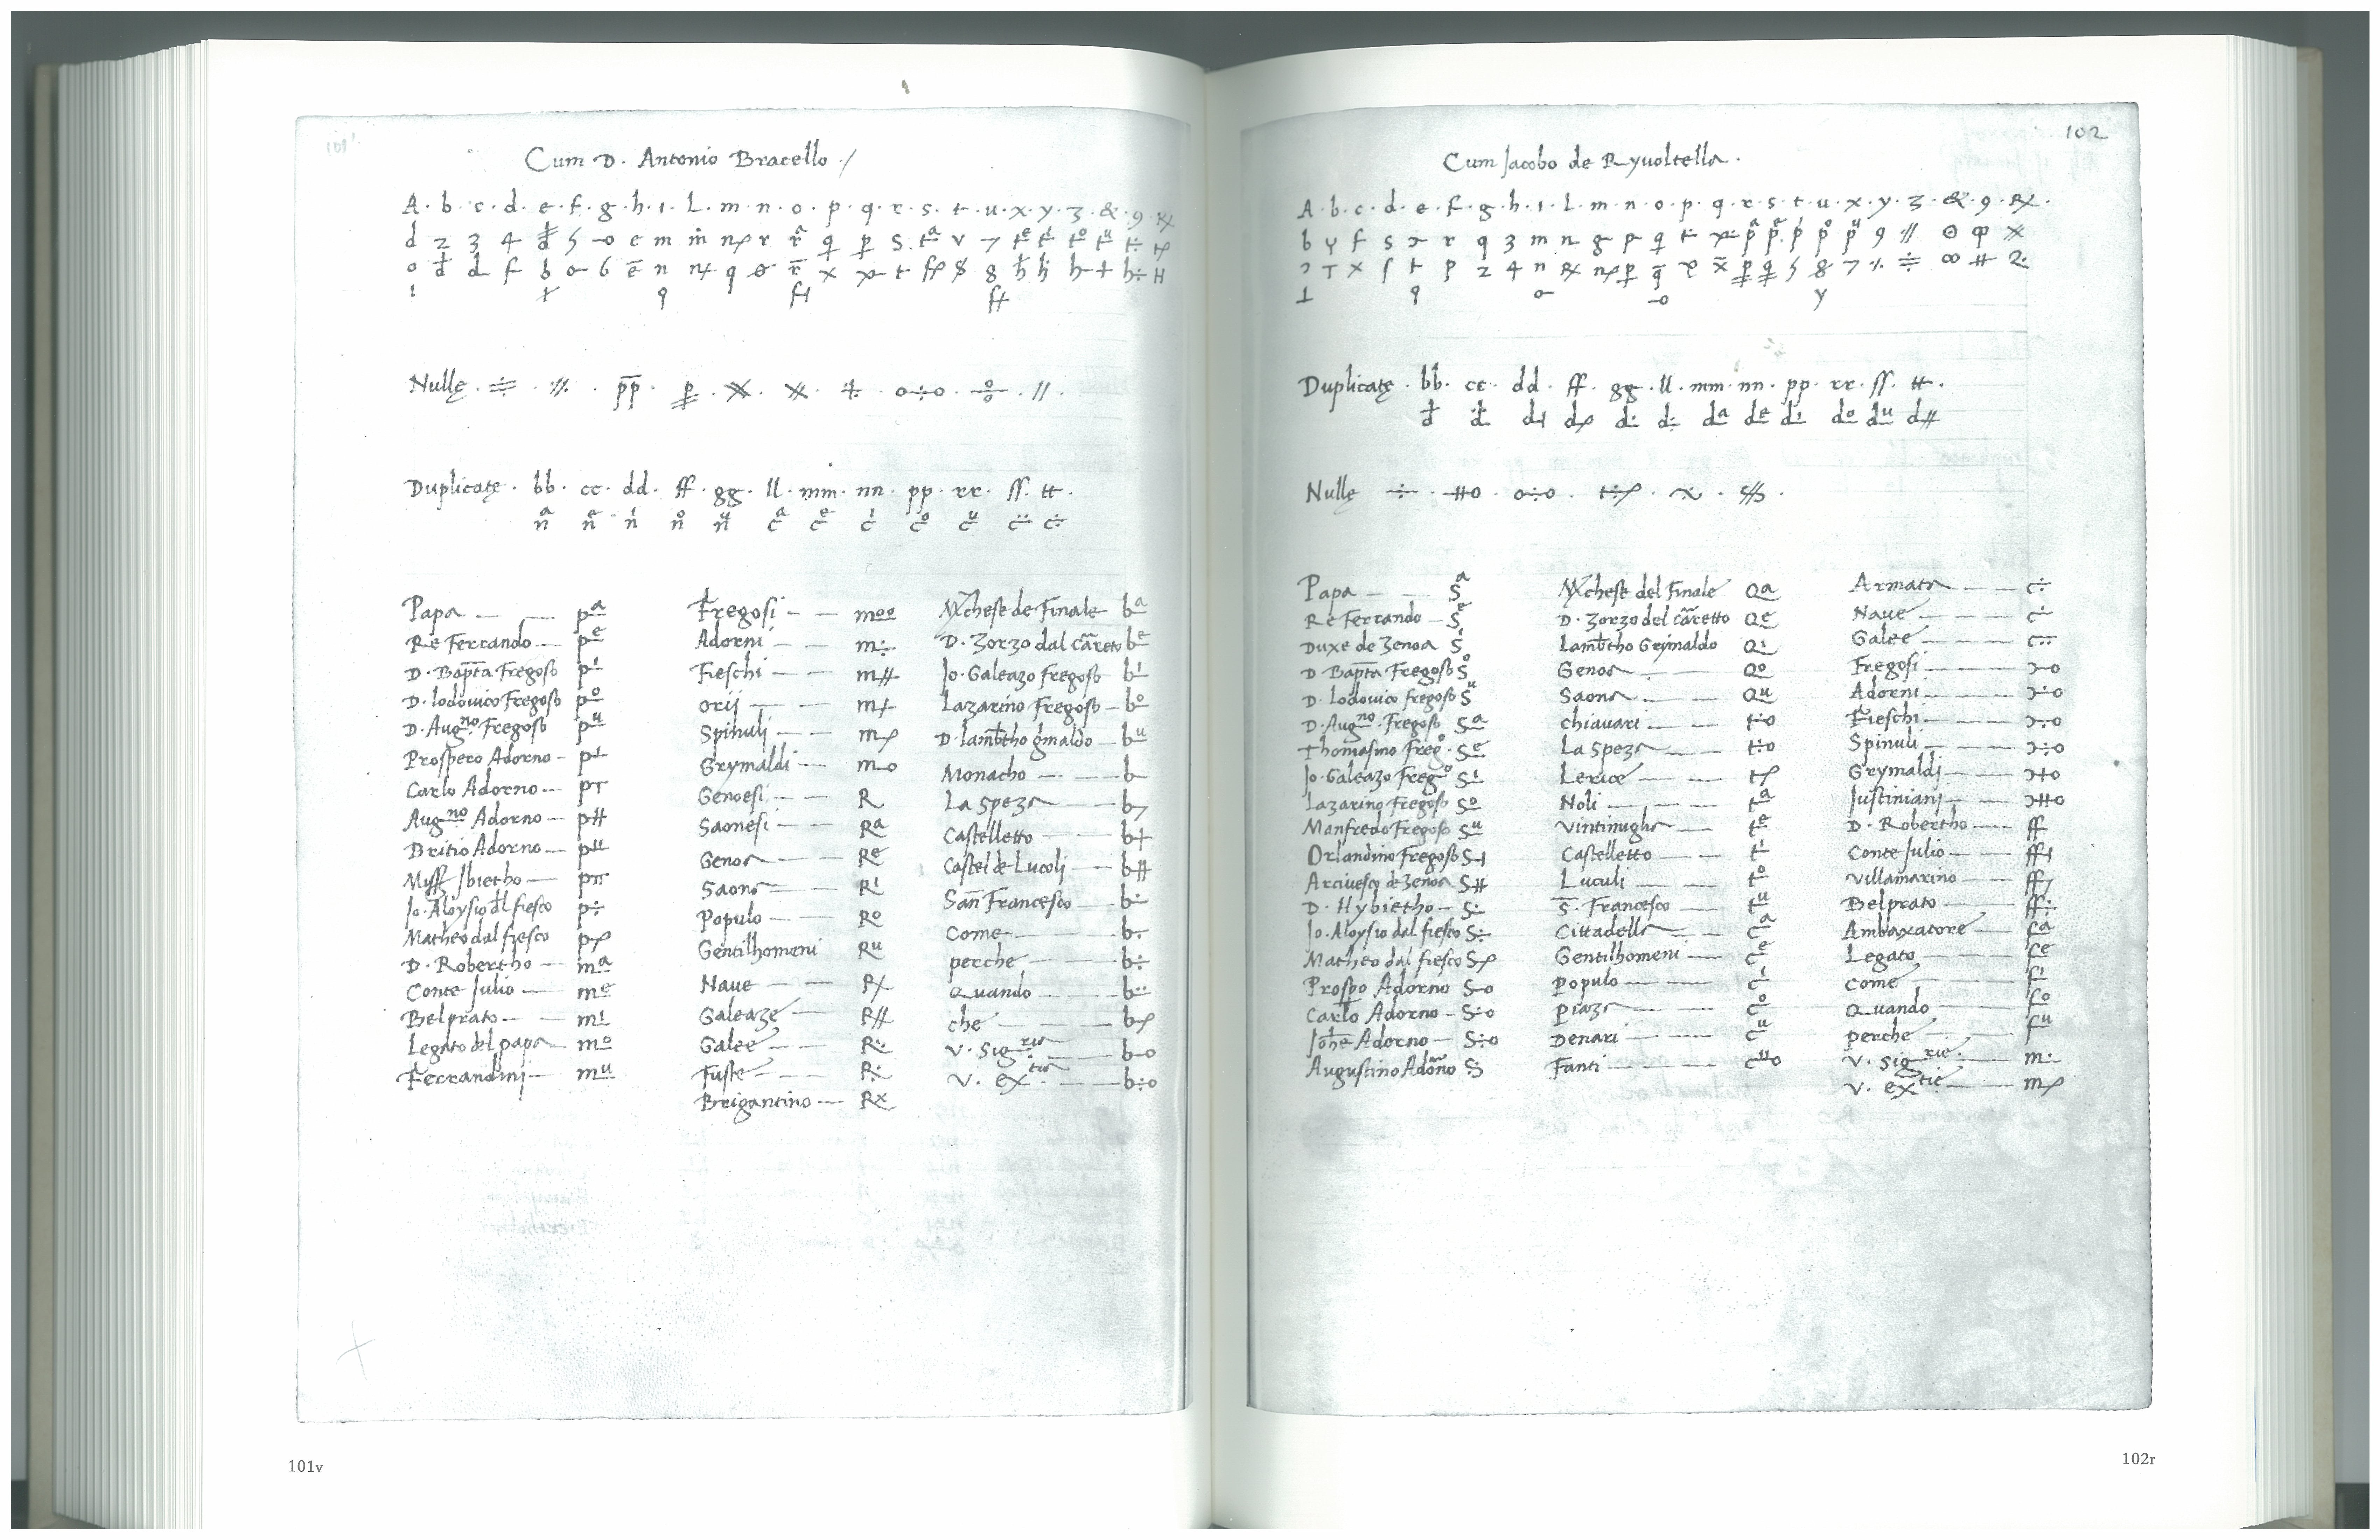
\includegraphics[width=0.95\textwidth]{img/img7.png}
                \caption{Ukážka nomenklátora z knihy \newline Francesco Tranchedino: Secret Diplomatic Documents \cite{tranchedino2011secret}}
                \label{fig:img7}
            \end{figure}
            \paragraph{Typy substitučných podsystémov v nomenklátoroch (písmená, n-gramy, klamáče, kódy)}
            \begin{table}[H]
                \centering
                \begin{tabular}{
                    >{\raggedright\arraybackslash}p{3cm} 
                    >{\raggedright\arraybackslash}p{5cm} 
                    >{\raggedright\arraybackslash}p{4cm}
                }
                    \toprule
                    \textbf{Typ} & \textbf{Charakteristika} & \textbf{Príklad} \\
                    \midrule
                    Písmená & Jednoduchá náhrada znakov & A~$\rightarrow$~X \\
                    N-gramy & Náhrada skupín znakov & TH~$\rightarrow$~WQ \\
                    Klamáče & Falošné znaky bez významu & *~$\rightarrow$~\ddag \\
                    Kódy & Slovné substitúcie & "Kráľ"~$\rightarrow$~"Z42" \\
                    \bottomrule
                \end{tabular}
                \caption{Typy substitúcií v nomenklátoroch}
            \end{table}
            
            Kľúče boli vizuálne štrukturované do tabuliek s:
            \begin{itemize}
                \item Vertikálnym usporiadaním pôvodných znakov
                \item Horizontálnymi riadkami pre šifrové ekvivalenty
            \end{itemize}
            \subsubsection{Substitučná šifra}
                Substitučné šifry nahradzujú každé písmeno abecedy jedným pevným zástupcom, pričom delenie slov zostáva nezmenené. Každý znak šifrovaného textu je priradený pravdepodobnosti, že reprezentuje konkrétne písmeno otvoreného textu, pričom tieto pravdepodobnosti sa aktualizujú na základe spoločných výskytov písmen \cite{ritter1990substitution}.
                
            \subsubsection{Jednoduchá substitučná šifra}
                Jednoduché substitučné šifry patria medzi šifrovacie metódy, v ktorých je každé písmeno otvoreného textu nahradené pevným písmenom šifrového textu, pričom medzery medzi slovami zostávajú zachované. Tento typ šifier sa často vyskytuje v novinových hlavolamoch a lúštiteľských úlohách \cite{olson2007robust}.
                
                Príklad šifry:
                
                    \begin{verbatim}
                        Pôvodná správa: abcdefghijklmnopqrstuvwxyz
                        Šifrovaná správa: qjzvukbymwphgxtlscnrfdoaie
                    \end{verbatim}
            \subsubsection{Monoalphabetická a homofónna substitúcia}
                Monoalphabetická substitúcia predstavuje spôsob šifrovania, pri ktorom je každému znaku otvoreného textu priradený vždy ten istý náhradný znak alebo symbol v šifrovom texte. Tento princíp znamená, že rovnaké písmeno sa v celom texte nahrádza identickým symbolom, čo však zároveň umožňuje využitie frekvenčnej analýzy na prelomenie šifry.
                Homofónna substitúcia je rozšírením monoalphabetickej substitúcie, pri ktorom môže byť jednému znaku otvoreného textu priradených viacero rôznych náhradných symbolov. Cieľom je potlačiť frekvenčné charakteristiky jazyka a sťažiť kryptanalýzu, keďže často sa vyskytujúce znaky môžu byť reprezentované viacerými alternatívami.
                V kontexte nomenklátorov sa homofónna substitúcia často využívala na šifrovanie najčastejších písmen alebo slabík \cite{kahn1996codebreakers}.
            \subsubsection{Bigramová a trigramová substitúcia}
                Bigramová substitúcia spočíva v nahrádzaní dvojíc znakov, teda bigramov, jedným symbolom alebo číselným označením. Podobne trigramová substitúcia pracuje s trojicami znakov.
                Použitie bigramov a trigramov zvyšuje efektivitu šifrovania, pretože umožňuje kódovať celé často sa opakujúce skupiny písmen namiesto jednotlivých znakov. V nomenklátoroch sa takýmto spôsobom často šifrovali bežné jazykové kombinácie, čím sa znižovala dĺžka výsledného šifrového textu a zároveň sa komplikovala jeho analýza \cite{kahn1996codebreakers}.
            \subsubsection{Kódové slová}
                Kódové slová predstavujú v nomenklátore špecifické výrazy, mená, miesta alebo často používané frázy, ktorým je priradený samostatný kód, najčastejšie vo forme čísla alebo symbolu.
                Na rozdiel od substitúcie jednotlivých znakov ide o nahrádzanie celých slov alebo pojmov. Tento prístup bol mimoriadne vhodný pri diplomatickej a vojenskej komunikácii, kde sa často opakovali rovnaké mená, geografické názvy alebo operačné termíny \cite{kahn1996codebreakers}.
            \subsubsection{Nully a doplnkové znaky}
                Nully a doplnkové znaky sú prvky šifrového textu, ktoré nenesú žiadny význam vo vzťahu k pôvodnej správe. Ich úlohou je zmiasť potenciálneho kryptanalytika a sťažiť rozpoznanie skutočnej štruktúry správy.
                Tieto znaky sa vkladali na náhodné pozície v texte alebo medzi významové časti správy. V nomenklátoroch sa používali najmä na narušenie frekvenčnej analýzy a zakrytie hraníc medzi jednotlivými kódovými prvkami \cite{kahn1996codebreakers}.
                 
    \subsection{Umelá inteligencia pre porozumenie rukou písaných dokumentov}
    Umelá inteligencia zohráva v súčasnej dobe zásadnú úlohu pri spracovaní historických a rukou písaných dokumentov. Proces digitalizácie archívnych materiálov, historických záznamov a rukopisov si vyžaduje automatické nástroje na analýzu veľkého množstva dát, čo je manuálne časovo veľmi náročné a často neefektívne. Pokročilé metódy založené na strojovom učení a hlbokých neurónových sieťach umožňujú efektívne identifikovať štruktúru dokumentov, lokalizovať textové prvky a spracovávať aj dokumenty, ktoré sú značne poškodené.

    Dôležitou súčasťou spracovania dokumentov je detekcia objektov v obraze, čo predstavuje základný krok k určeniu textových oblastí, symbolov či ďalších dôležitých prvkov obsiahnutých v materiáloch. Táto úloha je obzvlášť náročná pri historických rukou písaných dokumentoch, ktoré často vykazujú rôzne druhy poškodenia, nejednotný štýl písma, vizuálny šum alebo nízky kontrast.

    V ďalších podkapitolách sa rozoberajú princípy detekcie objektov, využitie konvolučných neurónových sietí na spracovanie obrazových údajov, ako aj špecifiká pri analýze rukopisov a historických materiálov obsahujúcich rukou písaný text.
        \subsubsection{Detekcia objektov v obraze}
            Detekcia objektov je kľúčová v oblasti počítačového videnia, ktorá pracuje na lokalizácii a identifikácii objektov v obrázkoch. Na rozdiel od segmentácie, ktorá rozdeľuje obraz na oblasti podľa triedy alebo podľa jednotlivých objektov, detekcia objektov označuje objekty pomocou ohraničujúcich rámčekov a priraďuje im triedu \cite{ultralytics_yolo11_detection}. V oblasti spracovania dokumentov sa detekcia používa na nájdenie blokov textu, hlavičiek, podpisov alebo pečiatok.
        \subsubsection{Princípy detekcie objektov}
        Moderné nástroje detekcie objektov využívajú hlboké neurónové siete. Tie sa dokážu
        sústrediť na relevantné vlastnosti obrázku a lokalizovať v ňom objekty. Detekcia objektov
        zvyčajne zahŕňa dva hlavné kroky: 
        \begin{itemize}
            \item lokalizácia – určenie polohy objektov v obraze pomocou ohraničujúcich rámčekov 
            \item klasifikácia – priradenie správnej triedy každému detegovanému objektu 
        \end{itemize}
        Klasické algoritmy, ako Viola-Jones, boli nahradené hlbokými modelmi, ktoré
        dosahujú vyššiu presnosť a robustnosť aj pri nekvalitnom osvetlení, šume či deformáciách
        dokumentov \cite{redmon2016yolo, ren2015faster}. 
        Konvolučné neurónové siete (CNN) pre detekciu objektov tvoria základ väčšiny moderných detekčných architektúr. Využívajú sa na extrakciu črt z obrázkov a následnú predikciu pozícií a tried objektov. Medzi najznámejšie architektúry patria napríklad:
            \begin{itemize}
                \item R-CNN a jeho varianty (Fast R-CNN, Faster R-CNN) \cite{girshick2014rcnn}
                \item YOLO (You Only Look Once) \cite{redmon2016yolo}
                \item SSD (Single Shot MultiBox Detector) \cite{liu2016ssd}
            \end{itemize}
        \subsubsection{Špecifiká spracovania rukou písaného textu}
        Rukou písaný text je pre umelú inteligenciu veľkou výzvou v porovnaní so strojovo tlačeným písmom. Každý človek píše inak, niekto má písmo uhladené, iný nečitateľné, niekto píše veľkými písmenami, ďalší píše kurzívou. Táto obrovská odlišnosť štýlov spôsobuje, že aj pre moderné AI systémy je rozpoznávanie rukopisov náročné.
        Ďalším problémom je, že znaky v rukopise často splývajú, najmä pri písaní kurzívou. Písmená môžu byť prepojené, čo sťažuje rozlíšenie, kde jedno písmeno končí a druhé začína. Ak je navyše text písaný nahusto alebo nepresne, systémy majú problém správne rozpoznať jednotlivé znaky.
        Rukou písané dokumenty sú často poškodené. Poškodenia obrázkov, ako napríklad škvrny alebo rozmazanosť, výrazne znižujú presnosť rozpoznávania.
        Napriek týmto prekážkam sa vďaka pokročilým technológiám presnosť rozpoznávania rukopisu stále zlepšuje, čo môže pomôcť pri digitalizácii historických archívov alebo rýchlejšiemu spracovaniu údajov.

\section{Analýza súčasného stavu a návrh riešenia}
Táto kapitola sa venuje analýze existujúcich prístupov k segmentácii a detekcii komponentov v historických rukou písaných šifrovacích kľúčoch. Najskôr sa zameriava na tradičné aj moderné metódy detekcie dokumentov a následne na využitie umelej inteligencie pri analýze historických dokumentov a šifier. Na základe tejto analýzy je zdôvodnený výber konkrétnej detekčnej architektúry a navrhnutý systém, ktorý je optimalizovaný pre potreby spracovania historických šifrovacích kľúčov.

    \subsection{Prehľad existujúcich prístupov k detekcii dokumentov}
    Detekcia prvkov dokumentov je dôležitým krokom pri spracovaní historických rukopisov a šifrovacích kľúčov. Táto sekcia sa zameriava na tradičné a moderné prístupy, ktoré sa používajú na rozdelenie dokumentov na jednotlivé časti. Následne zhodnotíme ich výhody a obmedzenia v kontexte historických dát.
    
        \subsubsection{Tradičné metódy (napr. založené na pravidlách, projekčných profiloch)}
        Tradičné metódy detekcie a segmentácie dokumentov sú základom automatizovaného spracovania obrazových dát. Tieto prístupy často využívajú jednoduché pravidlá, ako je detekcia okrajov, prahovanie, morfologické operácie alebo projekčné profily. Projekčný profil analyzuje rozloženie pixelov v riadkoch a stĺpcoch. To umožňuje identifikovať textové riadky alebo stĺpce v historických dokumentoch. Pravidlové metódy sú rýchle a výpočtovo nenáročné, no ich presnosť výrazne klesá pri zložitejších alebo poškodených dokumentoch, kde je veľká variabilita písma, šum alebo poškodenie papiera \cite{likforman2017text, casey1996survey}.
        \subsubsection{Metódy založené na strojovom učení a hlbokom učení}
        S rozvojom strojového a hlbokého učenia sa segmentácia a detekcia dokumentov posúva na novú úroveň. Konvolučné neurónové siete (CNN) dokážu automaticky extrahovať zložité črty z obrázkov a efektívne rozlíšiť rôzne komponenty dokumentov, ako sú textové bloky, tabuľky alebo špecifické znaky šifrovacích kľúčov \cite{oliveira2018dhsegment, xu2020layoutlm}. Hlboké učenie umožňuje modelom učiť sa priamo z veľkého množstva označených historických dát a adaptovať sa na rôzne štýly písma a štruktúry dokumentov \cite{simistira2017icdar, zhai2019deep}. Významným prínosom je aj možnosť trénovať modely na syntetických dátach, ktorými sú umelo generované údaje napodobňujúce charakteristiky a vzory reálnych údajov, čo zvyšuje ich odolnosť voči šumu a degradácii \cite{wigington2018start}.
    \subsection{Prehľad využitia AI pri analýze historických dokumentov a šifier}
    Umelá inteligencia sa dnes využíva na analýzu a spracovanie historických dokumentov vrátane šifrovacích kľúčov. Platformy ako Transkribus umožňujú automatickú transkripciu rukou písaných textov pomocou pokročilých modelov založených na rekurentných a konvolučných neurónových sieťach \cite{michael2018transkribus}. Tieto nástroje dokážu rozpoznať aj veľmi špecifické písma, adaptovať sa na rôzne jazyky a zvládnuť aj poškodené alebo neúplné zápisy. AI sa využíva nielen na rozpoznávanie samotného textu, ale aj na analýzu rozloženia stránky, detekciu prvkov, ako sú tabuľky, symboly alebo špecifické znaky kľúčov \cite{gruning2019read}. Moderné AI systémy tak značne urýchľujú a spresňujú výskum historických šifier a umožňujú efektívnu digitalizáciu archívov.
    \subsection{Voľba technológie pre detekciu}
    Pri výbere technológie pre detekciu častí historických rukou písaných šifrovacích kľúčov je potrebné zohľadniť rozličné druhy písma, prítomnosť šumu a potrebu detegovať rozličné objekty. Moderné detekčné architektúry založené na hlbokom učení, ako YOLO (You Only Look Once)\cite{redmon2016yolo}, ponúkajú vysokú presnosť pri spracovaní rôznych typov dát. YOLO je vhodné pre lokalizáciu a zaradenie viacerých objektov rôznych veľkostí v jednom kroku.
        \subsubsection{Zdôvodnenie výberu YOLO (You Only Look Once)}
        YOLO je jedným z najefektívnejších detekčných algoritmov v oblasti počítačového videnia. Hlavnou výhodou YOLO je schopnosť spracovať celý obraz naraz, čo výrazne zrýchľuje detekciu objektov. Algoritmus rozdeľuje obraz na mriežku a v každej bunke predikuje ohraničujúce obdĺžniky (bounding boxes) a pravdepodobnosti tried. Vďaka tomu dokáže detegovať aj malé objekty a je robustný voči rôznym šumom a deformáciám, čo je pri historických rukopisoch veľmi dôležité. YOLO je dobre dokumentovaný a existuje množstvo implementácií a predtrénovaných modelov, čo urýchľuje vývoj a testovanie \cite{redmon2016yolo}.
        \subsubsection{Predstavenie architektúry YOLO11}
        YOLO11 je v čase písania najnovšia generácia YOLO architektúry. Prináša ďalšie vylepšenia v presnosti, rýchlosti a efektivite spracovania. Vychádza z plne konvolučnej siete, kde základom je extraktor príznakov (Darknet-53 vo verzii YOLOv3, v novších verziách vylepšený backbone)\cite{redmon2018yolov3}. YOLO11 využíva pokročilé techniky:
        \begin{itemize}
            \item viacúrovňové feature fusion - spájanie malých prvkov z viacerých vrstiev do jedného
            \item vylepšené mechanizmy pre detekciu malých objektov
        \end{itemize}
        Vďaka tomu je vhodný aj na detekciu malých detailov v historických rukou písaných dokumentoch, kde je potrebné rozlišovať medzi rôznymi typmi znakov, symbolov a štruktúr.
    \subsection{Navrhovaný systém detekcie}
    Navrhovaný systém detekcie komponentov historických rukou písaných šifrovacích kľúčov je postavený na architektúre YOLO11. Dataset pozostáva z kľúčov, ktorých časti sú označené:
    \begin{itemize}
        \item element
        \item pair
        \item section
    \end{itemize}
    YOLO11 sa natrénuje na datasete. Výstupom sú váhy, ktoré sa dajú využiť na identifikáciu a klasifikáciu obrázkov predstavujúcich rovnakú problematiku. Tento prístup umožňuje efektívne spracovanie, automatizuje identifikáciu šifrovacích prvkov a výrazne zjednodušuje ďalšie kroky spracovania historických rukou písaných šifrovacích kľúčov.

\section{Príprava dátovej sady (Datasetu)}
Príprava kvalitného datasetu predstavuje dôležitý krok v úspešnom vývoji systému umelej inteligencie pre detekciu historických rukou písaných šifrovacích kľúčov. Táto kapitola detailne opisuje proces zhromažďovania a spracovania dát potrebných na trénovanie modelov hlbokého učenia. Osobitná pozornosť je venovaná špecifikám nomenklátorových šifier a ich charakteristikám. Tie tvoria základ pre definovanie tried pre detekciu. Proces anotácie je navrhnutý tak, aby zachytil štruktúru týchto jednotlivých tried. 
    \subsection{Zdroj a charakteristika dát}
    Zdrojom dát pre túto prácu sú historické rukou písané nomenklátorové šifrovacie kľúče pochádzajúce z viacerých zbierok. Tieto dokumenty predstavujú jedinečnú kategóriu kryptografických materiálov, ktoré kombinujú viacero substitučných mechanizmov. Nomenklátor ako rozšírená verzia jednoduchej substitučnej homofónnej šifry umožňuje využitie substitúcie jednotlivých písmen, n-gramov, klamáčov a špeciálnych kódov pre slová.
    
    Charakteristickou črtou týchto dokumentov je ich vizuálna štruktúra, kde jednotlivé substitučné podsystémy sú graficky oddelené a organizované do tabuľkových formátov. Substitúcie písmen sú typicky usporiadané do pravidelných mriežok, n-gramy do tabuliek, zatiaľ čo kódy pre celé slová môžu byť organizované vo formáte slovníka. Historické dokumenty tohto typu vykazujú značnú variabilitu v rukopise, kvalite papiera a stave zachovania, čo predstavuje výzvu pre spracovanie.
    
    Digitalizácia týchto dokumentov bola realizovaná vysokorozlišovacím skenovaním. Celková kolekcia zahŕňa dokumenty v rôznych jazykoch, predovšetkým v taliančine a latinčine, a môže sa v nej nachádzať terminológia z turečtiny, gréčtiny alebo slovanských jazykov, čo odráža diplomatickú prax daného obdobia.
    \subsection{Popis dátovej sady}
    Finálna dátová sada obsahuje 87 digitalizovaných strán historických nomenklátorových šifrovacích kľúčov, pričom každá strana predstavuje samostatnú jednotku pre detekciu. Každý obrázok zachytáva inú veľkosť a množstvo elementov, čo prispieva k rôznorodosti datasetu.
    Dokumenty obsahujú hlavné typy substitučných podsystémov, ktorými sú písmená, n-gramy, klamáče a kódy. Dataset odráža historickú realitu používania týchto šifier v praxi.
    Kvalita dokumentov sa pohybuje od výborne zachovaných exemplárov s čitateľným rukopisom až po degradované materiály s presvitajúcimi stranami. Keďže ide o skeny, model YOLO sa bude musieť pri trénovaní vysporiadať s týmito nedostatkami.
    \subsection{Anotácia dát}
    Anotácia dát je zásadným krokom pri príprave datasetu na trénovanie modelov detekcie objektov. Kvalita týchto anotácií výrazne ovplyvňuje schopnosť modelu presne lokalizovať a klasifikovať objekty v dokumentoch. V rámci tejto práce bolo potrebné identifikovať a definovať vhodné triedy objektov, ktoré reprezentujú jednotlivé časti nomenklátorových šifrovacích kľúčov, a následne vykonať manuálnu anotáciu historických dokumentov s využitím špecializovaných nástrojov.

    Nasledujúce podkapitoly sa zameriavajú na podrobný opis výberu tried objektov, proces anotácie a spracovanie datasetu.
        \subsubsection{Definovanie tried pre detekciu objektov}
        Pre potrebu detekcie častí nomenklátorových šifrovacích kľúčov boli definované tri hlavné triedy, ktoré zachytávajú všetky relevantné komponenty týchto historických dokumentov.

        Trieda " element" predstavuje jednotlivé elementy. Môžu to byť slová, slabiky alebo písmená, ktoré môžu vyjadrovať:
        \begin{itemize}
            \item názov sekcie
            \item kódové slovo
            \item substitučný symbol
        \end{itemize}
         Táto trieda zachytáva základné stavebné kamene šifrovacích kľúčov, ktoré sú nevyhnutné na pochopenie ich štruktúry. Táto trieda bola v datasete najčastejšie zastúpená.
        
        Trieda "pair" zachytáva pridruženie kódového slova k substitučnému symbolu. Nie každý element však má svoj pár.
        
        Trieda "section" predstavuje ohraničujúce sekcie, ktoré rozdeľujú jednotlivé časti kľúča.
  
            \begin{figure}[H]
                \centering
                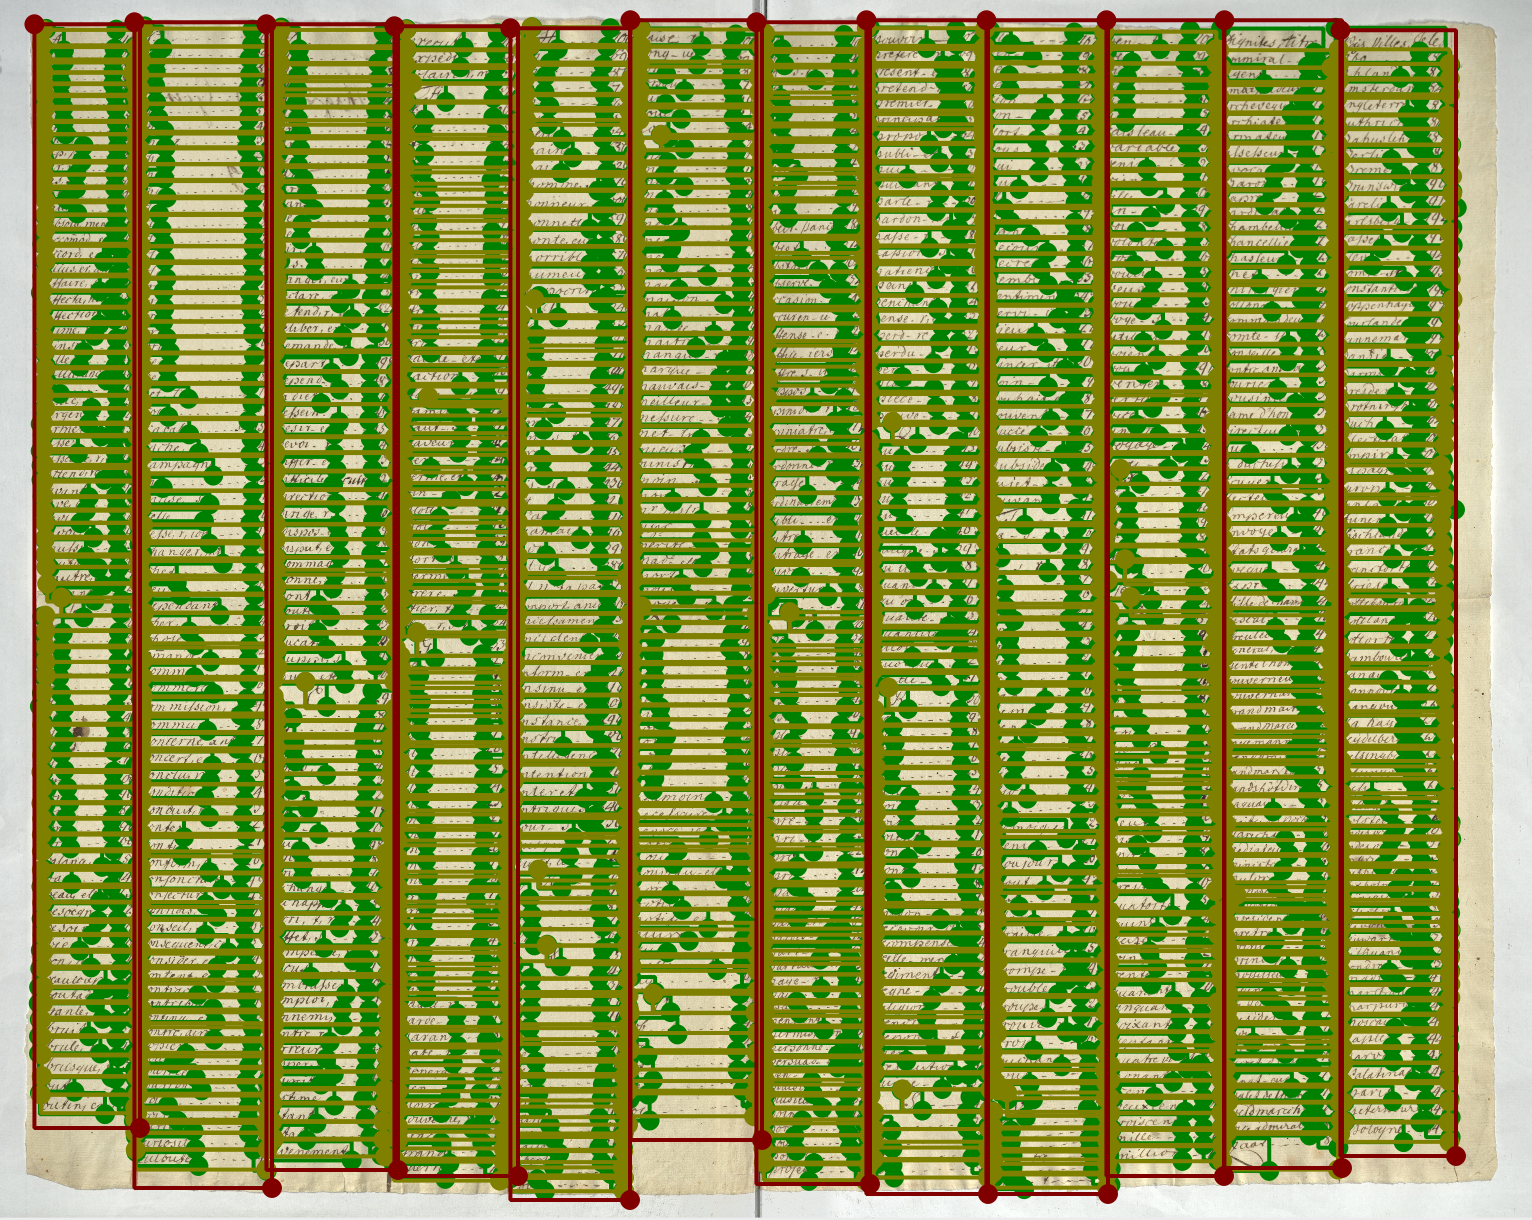
\includegraphics[width=0.95\textwidth]{img/dataset_ukazka.png}
                \caption{Ukážka obrázku z datasetu HLA–HStAM, Best. 4d, (c) HLA–HStAM, f. 4d, Nr. 1220 \cite{HLA1220}}
                \label{fig:dataset_ukazka}
            \end{figure}
            \begin{figure}[H]
                \centering
                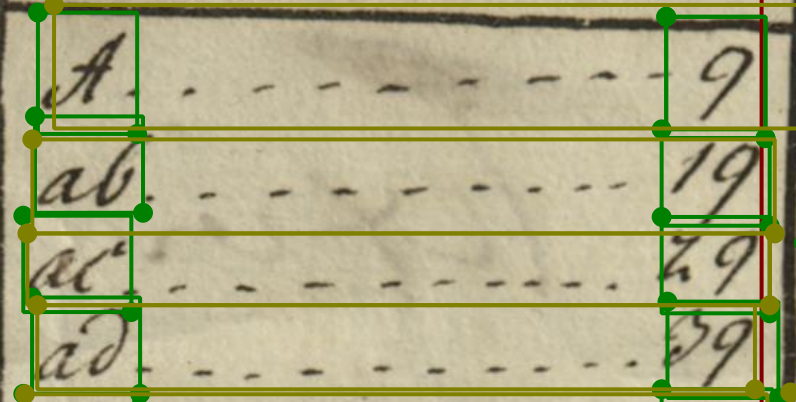
\includegraphics[width=0.95\textwidth]{img/dataset_closer.png}
                \caption{Ukážka obrázku z datasetu HLA–HStAM, Best. 4d, (c) HLA–HStAM, f. 4d, Nr. 1220 \cite{HLA1220} s detailnejším pohľadom na anotované objekty}
                \label{fig:dataset_closer}
            \end{figure}
            \begin{figure}[H]
                \centering
                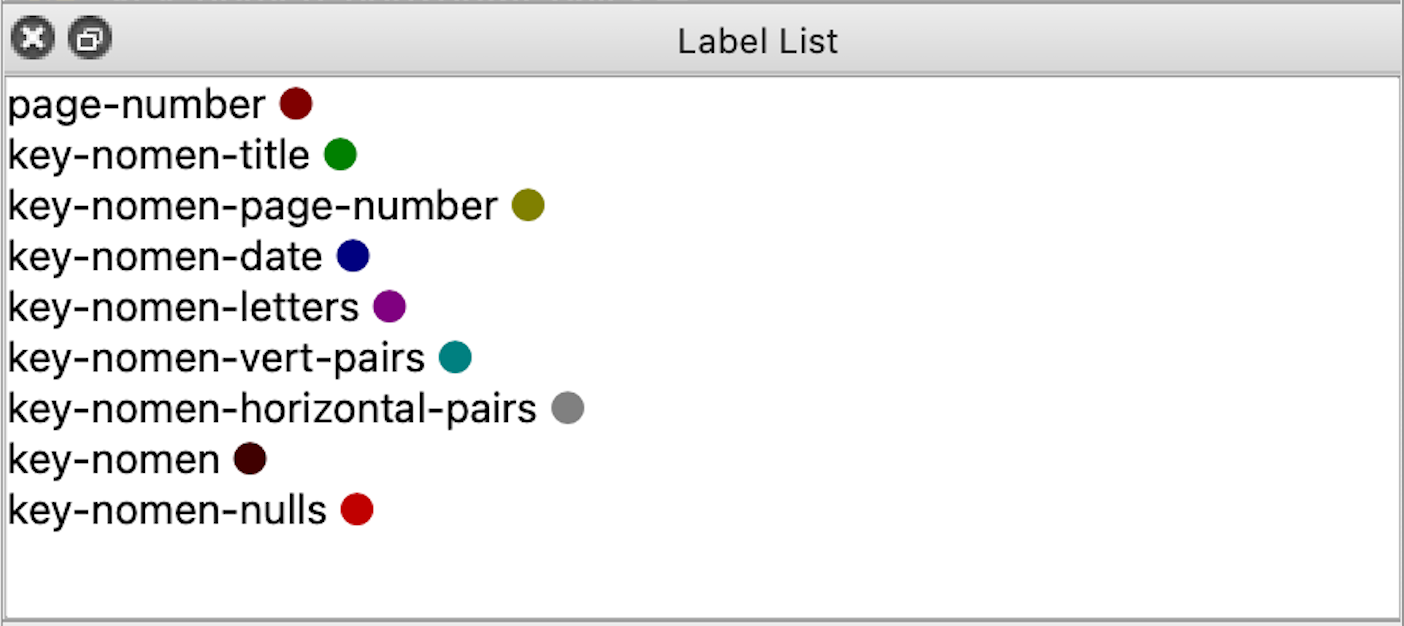
\includegraphics[width=0.95\textwidth]{img/labels.png}
                \caption{Legenda k označeniu sekcií}
                \label{fig:labels}
            \end{figure}
            \begin{figure}[H]
                \centering
                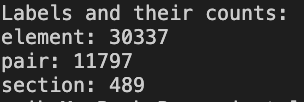
\includegraphics[width=0.95\textwidth]{img/count.png}
                \caption{Počet zastúpení jednotlivých tried v datasete}
                \label{fig:counts}
            \end{figure}
        
        \subsubsection{Proces a nástroje anotácie}
        Anotačný proces bol realizovaný pomocou špecializovaného nástroja labelme, ktorý umožňuje presné vymedzenie polygonálnych oblastí na dokumentoch a ich kategorizáciu podľa definovaných tried.
        
        Anotácia bola vykonávaná ručne. Každý dokument bol nezávisle anotovaný s následnou konzultáciou. Tento prístup zabezpečil vysokú kvalitu a spoľahlivosť anotácií, čo je kritické pre úspešné trénovanie modelov umelej inteligencie.
        
        Proces anotácie zahŕňal kroky, ktoré mali zabezpečiť validáciu kvality. Prvým krokom bola kontrola kompletnosti anotácií, pri ktorej sa overovalo, že všetky relevantné oblasti dokumentu sú označené a žiadna trieda nie je vynechaná.
    \subsection{Rozdelenie dátovej sady}
    Dátová sada bola rozdelená na trénovaciu a validačnú množinu v pomere 80:20. Trénovacia množina obsahuje 69 dokumentov a slúži na optimalizáciu parametrov neurónových sietí. Validačná množina s 18 dokumentmi je používaná na ladenie hyperparametrov a monitorovanie procesu trénovania s cieľom predchádzať pretrénovaniu. Testovacia množina s 18 dokumentmi zostáva počas celého procesu vývoja nedotknutá a slúži na finálne vyhodnotenie výkonnosti modelov.
    
    Rozdelenie bolo realizované skriptom poskytnutým samotným YOLO (labelme2yolo), aby sa zabezpečilo kompatibilné a rovnomerné zastúpenie dokumentov.
    \subsection{Predspracovanie a augmentácia dát}
    Kvalita vstupných dát patrí medzi kľúčové faktory, ktoré výrazne ovplyvňujú úspešnosť modelov strojového učenia pri spracovaní historických dokumentov. Tieto rukopisy často vykazujú rôzne znaky poškodenia, ako sú degradovaný materiál, šum, poškodenie papiera, nerovnomerné osvetlenie alebo nízka kontrastnosť textu. Tieto aspekty môžu podstatne zhoršiť presnosť detekcie objektov a rozpoznávanie textu, čo si vyžaduje dôkladný prístup k príprave údajov.

    Preto bolo nevyhnutné sústrediť sa na precízne predspracovanie datasetu ešte pred samotným trénovaním modelov. Hlavným cieľom predspracovania bolo dosiahnuť jednotný formát dokumentov, zvýrazniť relevantné štruktúry a minimalizovať negatívny vplyv rôznych typov degradácie, ktorými historické materiály často trpia. Tento krok priamo prispel k efektívnejšiemu učeniu neurónových sietí.

    Experimenty zahŕňali aj použitie techniky dátovej augmentácie, ktorá umožňuje rozšíriť trénovací dataset prostredníctvom rozličných transformačných metód. Augmentácia je obzvlášť dôležitá pri práci s menšími dátovými množinami, kde pomáha zlepšiť schopnosť modelu generalizovať a zároveň zvyšuje jeho odolnosť voči zmene vlastností vstupných dát.

    V nasledujúcich podkapitolách je podrobne rozpracovaný postup analýzy pôvodného datasetu, proces binarizácie historických dokumentov a aplikované techniky augmentácie dát.
        \subsubsection{Pôvodná podoba datasetu}
        Pôvodné digitalizované dokumenty sa nachádzali v rôznych formátoch a kvalitách, čo vyžadovalo štandardizáciu pre potreby trénovania neurónových sietí. Dokumenty boli pôvodne naskenované v rozlíšení 4k, s farebnými profilmi RGB a občasne aj v odtieňoch sivej. Súborové formáty zahŕňali JPEG a PNG so zväčša rovnakým rozlíšením.
    
        Prvým krokom predspracovania bola konverzia všetkých obrazov do jednotného formátu PNG bez kompresie, aby sa predišlo stratám kvality. Farebné obrazy boli v tejto fáze zachované pre možnú analýzu farebných charakteristík atramentov a papiera.
        \subsubsection{Binarizácia dát}
        Binarizácia predstavuje spôsob spracovania, ktorý transformuje farebné alebo sivé obrazy na čiernobiele reprezentácie, kde text a grafické elementy sú oddelené od pozadia. Pre historické dokumenty s degradáciou a nerovnomerným osvetlením preukázala výnimočnú účinnosť pri spracovaní degradovaných rukopisov. Tento prístup zabezpečil optimálnu kvalitu binarizácie pre špecifické charakteristiky týchto dokumentov. Binarizácia bola vykonaná viackrát, keďže vyhodnotenie šumu nebolo vždy úspešné.

        \begin{figure}[H]
            \centering
            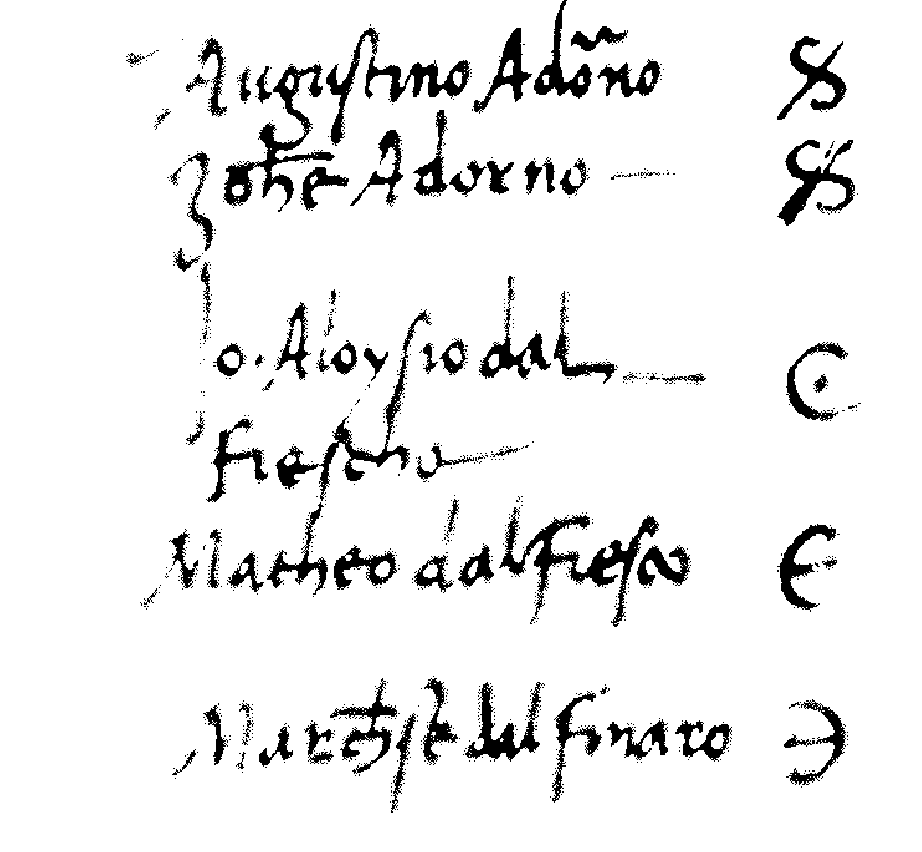
\includegraphics[width=0.95\textwidth]{img/bin_wrong.png}
            \caption{Binarizácia kde sa okrem šumu odstránili aj časti slova z knihy Francesco Tranchedino: Secret Diplomatic Documents \cite{tranchedino2011secret}}
            \label{fig:bin_wrong}
        \end{figure}

        \begin{figure}[H]
            \centering
            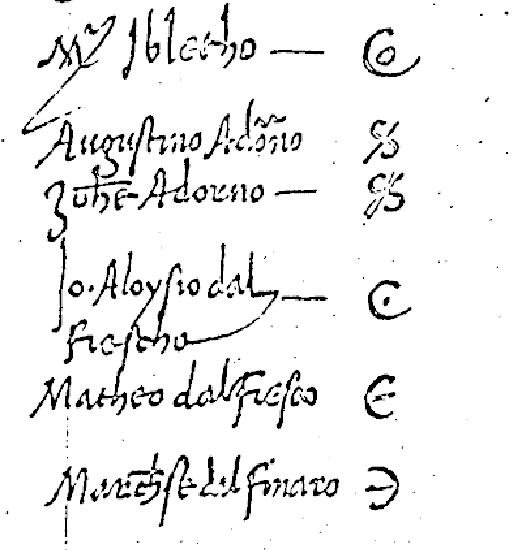
\includegraphics[width=0.95\textwidth]{img/bin_right.png}
            \caption{Binarizácia kde sa šum odstránil a slovo zostalo čitateľné z knihy Francesco Tranchedino: Secret Diplomatic Documents \cite{tranchedino2011secret}}
            \label{fig:bin_right}
        \end{figure}

        \subsubsection{Augmentácia dát}
        Augmentácia dát predstavuje techniku na zvýšenie rozmanitosti trénovacej množiny a zlepšenie generalizačnej schopnosti modelov, čo je obzvlášť dôležité pri relatívne malých datasetoch historických dokumentov. Implementovaná bola komplexná sada augmentačných techník špeciálne navrhnutých pre charakteristiky rukou písaných historických dokumentov.
        
        \begin{figure}[H]
            \centering
            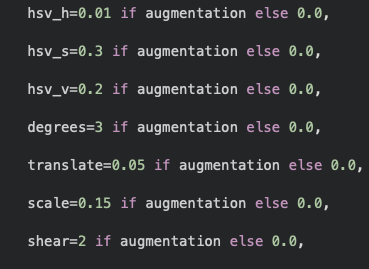
\includegraphics[width=0.95\textwidth]{img/aug.png}
            \caption{Časť kódu pre augmentáciu dat}
            \label{fig:aug_code}
        \end{figure}

\section{Implementácia a experimenty}
V tejto kapitole je popísaný proces implementácie a experimentálneho overenia detekčných modelov na úlohe detekcie komponentov historických rukou písaných nomenklátorových šifrovacích kľúčov. Cieľom experimentov bolo porovnať výkonnosť rôznych variantov modelu YOLO na viacerých verziách datasetu (pôvodný, binarizovaný, augmentovaný) a vyhodnotiť vplyv jednotlivých spracovaní na presnosť detekcie. Kapitola sa venuje výberu nástrojov,  konfigurácii modelov, nastaveniu tréningových parametrov, priebehu tréningu a použitiu hodnotiacich metrík.

    \begin{figure}[H]
        \centering
        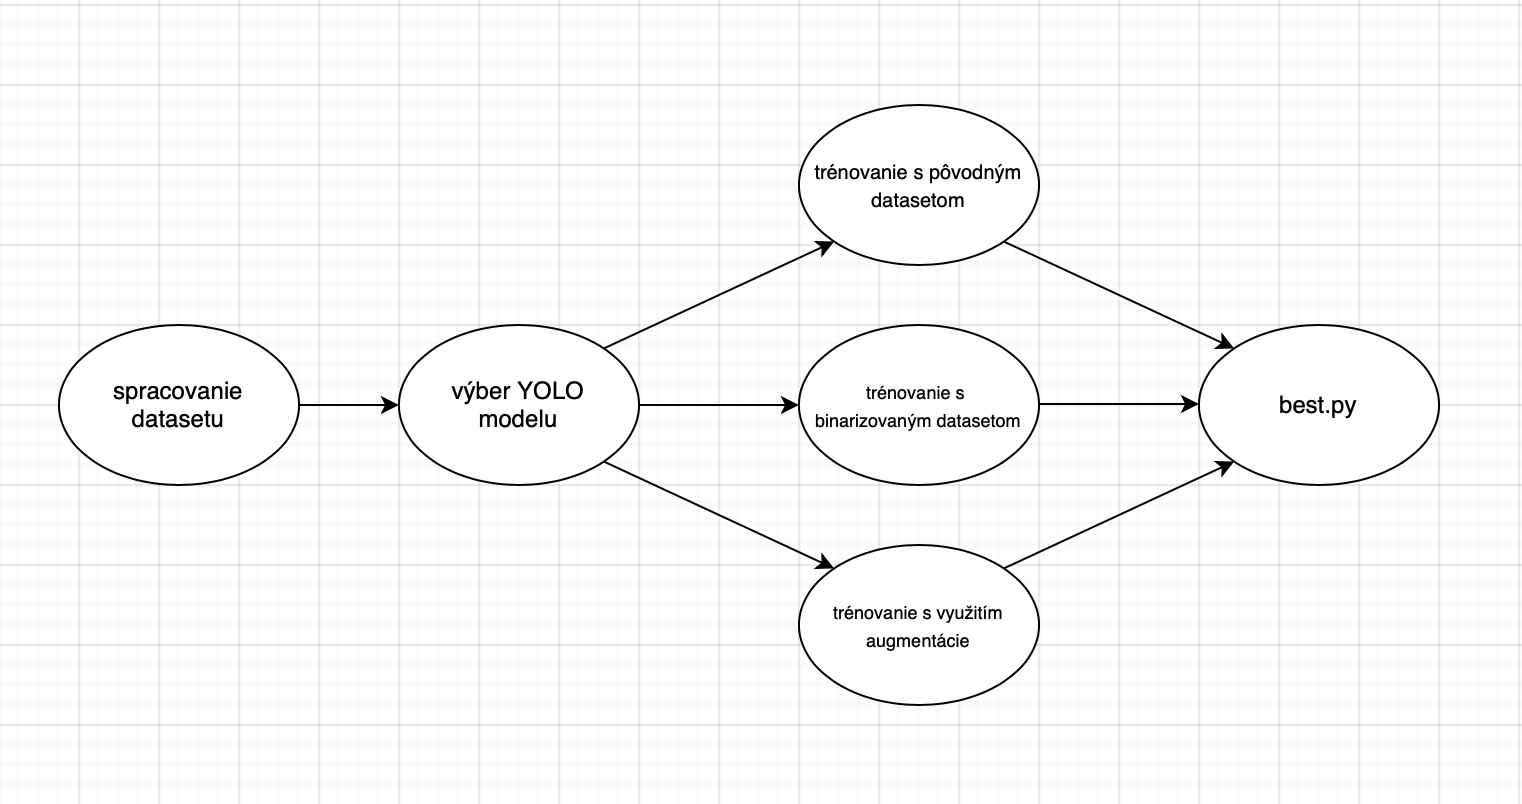
\includegraphics[width=0.95\textwidth]{img/diagram.png}
        \caption{Znázornenie postupu vyhodnocovania}
        \label{fig:aug_code}
    \end{figure}

\subsection{Použité nástroje a prostredie}
    Na implementáciu a experimentovanie boli využité open-source nástroje a knižnice pre spracovanie obrazu a trénovanie hlbokých neurónových sietí. Hlavným frameworkom bol PyTorch v kombinácii s knižnicou Ultralytics\cite{ultralytics2023yolo} YOLO11, ktorá poskytuje optimalizované implementácie najnovších architektúr YOLO. Pre anotáciu a vizualizáciu výsledkov boli použité vlastné skripty v Python 3.11.
    
    Výpočtové experimenty prebiehali na zariadení s grafickou kartou NVIDIA TESLA T4 (16GB VRAM). Tento hardvér umožnil efektívny tréning aj najväčších variantov modelu YOLO11 v krátkom čase.
    
    Pre binarizáciu datasetu boli využité knižnice OpenCV, shutil a glob. Augmentácia bola realizovaná pomocou YOLO priamo pri trénovaní.
    
    V rámci experimentov boli testované všetky hlavné varianty
    YOLO11:
    \begin{itemize}
        \item YOLO11n (nano)
        \item YOLO11s (small)
        \item YOLO11m (medium)
        \item YOLO11l (large)
        \item YOLO11x (extra large)
    \end{itemize}
    Každý model bol testovaný na identických dátových sadách, aby bolo možné objektívne porovnať ich výkonnosť.
    \subsection{Konfigurácia modelu YOLO11}
    Model YOLO11 je v čase písania tejto práce najnovšou generáciou objektových detektorov, ktorá prináša výrazné zlepšenia v rýchlosti a presnosti oproti predchádzajúcim verziám. Pre potreby tejto práce bola použitá konfigurácia pre úlohu detekcie objektov s viactriedovou segmentáciou podľa definovaných tried.

    Každý variant modelu bol inicializovaný s predtrénovanými váhami na COCO datasete, pričom následne prebiehal fine-tuning na vlastnej dátovej sade historických dokumentov. V rámci konfigurácie boli upravené nasledovné parametre: 
    
    \begin{itemize}
        \item Počet tried: 3 (element, pair, section)
        \item Vstupná veľkosť obrázkov: 640px-960px (downsamplované z pôvodných skenov, obmedzený kapacitou GPU pri väčších modeloch)
        \item Batch size: 2-8 (obmedzený kapacitou GPU pri väčších modeloch)
    \end{itemize}
    
    Konfiguračné súbory boli spravované pomocou nástroja labelme2yolo do formátu YAML. Labelme2yolo tiež štandardne prerozdelilo dataset pre tréning a validáciu dát.

    \subsection{Tréningové parametre}
    Tréning modelov prebiehal v niekoľkých fázach. Hlavnými premennými boli počet epoch, veľkosť batchu, vstupná veľkosť obrázkov a samotný výber modelu. Pre každý variant modelu a každú verziu datasetu (pôvodný, binarizovaný, augmentovaný) bolo experimentálne nastavené rozmedzie na 30-300 epoch. Počiatočné tréningy boli realizované na 30-70 epoch, pričom na základe priebehu validačnej straty bol počet epoch zvyšovaný až do dosiahnutia optimálneho výkonu. Nižší počet epoch slúžil na výber správneho modelu.

    Patience je argument pri spustení trénovania, ktorý pri stagnácii zastaví trénovanie. Tým sa eliminuje problém pretrénovania. Argument batch určuje počet obrázkov spracovaných modelom počas jednej iterácie tréningu pred aktualizáciou váh neurónovej siete\cite{ultralytics_batch}.
    \subsection{Výber modelu}
            Prvý experimentálny scenár zahŕňal tréning modelov na pôvodných farebných digitalizovaných dokumentoch bez ďalšieho predspracovania. Cieľom bolo zistiť, do akej miery si model dokáže poradiť s variabilitou šumu a degradácie papiera. Následne sa sledoval vplyv veľkosti modelu na schopnosť učiť sa z týchto komplexných dát. Na základe výsledkov sa vybral model, ktorý sa bude ďalej testovať na datasete.
    
            Výsledky ukázali, že menšie modely (yolo11n.pt, yolo11s.pt) boli schopné naučiť sa požadované vzory. Ich menšia veľkosť vytvorila priestor pre vyššie hodnoty hyperparametrov, čím sa dokázali v efektívnosti vyrovnať väčším modelom.
            
            Stredné a veľké modely (yolo11m.pt, yolo11l.pt, yolo11x.pt), napriek ich veľkosti, nedosiahli väčšiu presnosť. Ich tréning bol náchylnejší na pretrénovanie a vzhľadom na ich náročnosť sa musela pamäť uvoľniť znížením hodnôt premenných, ktoré zefektívnili trénovanie na menších modeloch.
            
            Po zvýšení počtu epoch a aktivácií early stoppingu sa však podarilo dosiahnuť stabilnejšie výsledky.
            \subsubsection{YOLO11n}
            Model YOLO11n predstavuje najmenší variant architektúry YOLO11, navrhnutý primárne pre aplikácie s nízkymi hardvérovými nárokmi a požiadavkou na rýchlu inferenciu. Vyniká minimálnym počtom parametrov zo všetkých testovaných verzií, čo ho robí vhodným na implementáciu na menej výkonných zariadeniach alebo v prípadoch, kde je potrebná vysoká rýchlosť spracovania dát.

            V rámci experimentov bol tento model testovaný s vyšším vstupným rozlíšením obrázkov (imgsz=960) s cieľom zistiť, či zvýšenie rozlíšenia dokáže kompenzovať jeho obmedzenú kapacitu pri detekcii malých objektov. Vyššie rozlíšenie síce prispelo k zachovaniu jemných detailov, avšak samotná architektonická jednoduchosť modelu nepostačovala na efektívne zvládanie zložitejších dokumentových strán s veľkým počtom objektov.

            Výsledky ukázali nižšie hodnoty mAP50 aj recallu v porovnaní s robustnejšími variantmi modelu. To naznačuje, že príliš redukovaná architektúra nie je vhodným riešením pre úlohy zahŕňajúce husté súbory malých objektov. Hlavným prínosom zostáva nízka výpočtová náročnosť a krátky čas tréningu, čo však prichádza za cenu nižšej presnosti pri detekcii.
            \begin{table}[H]
            \centering
            \begin{tabular}{|l|c|}
                \hline
                \textbf{Parameter} & \textbf{Hodnota} \\ \hline
                Počet tried & 3 \\ \hline
                Počet tréningových obrázkov & 69 \\ \hline
                Počet validačných obrázkov & 18 \\ \hline
                Počet epoch & 50 \\ \hline
                Veľkosť obrázkov & 960 \\ \hline
                Batch size & 4 \\ \hline
                Použitý model & YOLO11n \\ \hline
                mAP@0.5 & 0.505 \\ \hline
                mAP@0.5:0.95 & 0.285 \\ \hline
                Precision & 0.803 \\ \hline
                Recall & 0.519 \\ \hline
            \end{tabular}
            \caption{Výsledky modelu YOLO11n}
            \label{tab:yolo11n}
            \end{table}

            \subsubsection{YOLO11s}
            Model YOLO11s predstavuje menší až stredne veľký variant architektúry YOLO11, ktorý ponúka vyváženú kombináciu medzi presnosťou detekcie, stabilitou tréningu a nárokmi na hardvér. Počas testovania preukázal vynikajúce celkové výsledky z hľadiska mAP50 a recallu.

            V porovnaní s väčšími modelmi sa ukázal ako stabilnejší počas tréningového procesu a zanechal menšiu stopu na využití GPU pamäte. Zároveň si model efektívne poradil so všetkými sledovanými triedami bez výrazného poklesu presnosti pri ktoromkoľvek type objektu. Mimoriadne cennou vlastnosťou bola jeho vysoká hodnota recallu, čo potvrdzuje schopnosť spoľahlivo detegovať väčšinu objektov v obraze.

            Hoci pri najkomplexnejšej triede „element“ nedosiahol najvyšší výkon, celkovo ponúkol najlepší kompromis medzi presnosťou a efektívnosťou. Vďaka týmto vlastnostiam bol model YOLO11s vyhodnotený ako najperspektívnejší kandidát pre ďalšie experimenty aj finálne nasadenie.
            \begin{table}[H]
                \centering
                \begin{tabular}{|l|c|}
                \hline
                \textbf{Parameter} & \textbf{Hodnota} \\ \hline
                Počet tried & 3 \\ \hline
                Počet tréningových obrázkov & 69 \\ \hline
                Počet validačných obrázkov & 18 \\ \hline
                Počet epoch & 50 \\ \hline
                Veľkosť obrázkov & 640 \\ \hline
                Batch size & 8 \\ \hline
                Použitý model & YOLO11s \\ \hline
                mAP@0.5 & 0.583 \\ \hline
                mAP@0.5:0.95 & 0.369 \\ \hline
                Precision & 0.867 \\ \hline
                Recall & 0.587 \\ \hline
                \end{tabular}
                \caption{Výsledky modelu YOLO11s}
                \label{tab:yolo11s}
            \end{table}

            \subsubsection{YOLO11m}
            Model YOLO11m predstavuje stredne veľký variant architektúry YOLO11, ktorý disponuje väčším počtom parametrov a vyššou schopnosťou učiť sa komplexné reprezentácie. Predpokladalo sa, že táto zväčšená verzia prinesie výraznejšie zlepšenie pri detekcii hustých a malých objektov. 

            Experimentálne výsledky však ukázali iba nepatrné zlepšenie pri kategóriách „pair“ a „element“, pričom celkové metriky zostali takmer totožné s menším modelom YOLO11s. Navyše sa prejavila vyššia výpočtová náročnosť tréningu a zvýšené požiadavky na GPU pamäť. Pri vyšších dávkach (batch size) často dochádzalo k preťaženiu pamäte GPU, čo spôsobovalo prechod niektorých operácií na procesor (CPU), a tým spomaľovalo celý tréningový proces.

            Tieto výsledky naznačujú, že samotné zväčšenie modelu nemusí byť zárukou výrazného zlepšenia kvality detekcie, najmä pri použití menších datasetov. Z tohto dôvodu nereprezentoval model YOLO11m výrazný posun vpred, a to vzhľadom na zvýšené nároky na hardvérové zdroje.           
            \begin{table}[H]
            \centering
                \begin{tabular}{|l|c|}
                \hline
                \textbf{Parameter} & \textbf{Hodnota} \\ \hline
                Počet tried & 3 \\ \hline
                Počet tréningových obrázkov & 69 \\ \hline
                Počet validačných obrázkov & 18 \\ \hline
                Augmentácia & Áno \\ \hline
                Počet epoch & 50 \\ \hline
                Veľkosť obrázkov & 640 \\ \hline
                Batch size & 4 \\ \hline
                Použitý model & YOLO11m \\ \hline
                mAP@0.5 & 0.567 \\ \hline
                mAP@0.5:0.95 & 0.333 \\ \hline
                Precision & 0.858 \\ \hline
                Recall & 0.574 \\ \hline
                \end{tabular}
                \caption{Výsledky modelu YOLO11m}
                \label{tab:yolo11m}
            \end{table}

            \subsubsection{YOLO11l}
            Model YOLO11l patrí k robustnejším verziám architektúry YOLO11, pričom jeho kapacita výrazne prevyšuje modely YOLO11s a YOLO11m. V testoch dosiahol najlepšie výsledky pri triedach „pair“ a „element“, ktoré sa vyznačovali najvyššou náročnosťou z hľadiska veľkosti objektov a ich hustoty v dátach.

            Zvýšená kapacita modelu umožnila presnejšiu identifikáciu komplexných vzorov a zachytenie jemných detailov objektov. Napriek týmto výhodám celkový výkon modelu vo väčšine prípadov výrazne neprevyšoval výsledky dosiahnuté menším modelom YOLO11s. Súčasne však došlo k výraznému nárastu hardvérových nárokov, najmä pokiaľ ide o využitie GPU pamäte a dĺžku tréningu.

            YOLO11l predstavuje vhodný nástroj pre situácie, kde je prioritná maximálna presnosť detekcie malých a hustých objektov, pod podmienkou dostupnosti výkonného hardvéru. V praktických aplikáciách však dodatočný výkon oproti modelu YOLO11s nebol natoľko výrazný, aby plne ospravedlnil vyššie požiadavky na výpočtové zdroje, a teda obmedzenie vstupných parametrov.
            \begin{table}[H]
                \centering
                
                \begin{tabular}{|l|c|}
                \hline
                \textbf{Parameter} & \textbf{Hodnota} \\ \hline
                Počet tried & 3 \\ \hline
                Počet tréningových obrázkov & 69 \\ \hline
                Počet validačných obrázkov & 18 \\ \hline
                Počet epoch & 50 \\ \hline
                Veľkosť obrázkov & 640 \\ \hline
                Batch size & 2 \\ \hline
                Použitý model & YOLO11l \\ \hline
                mAP@0.5 & 0.573 \\ \hline
                mAP@0.5:0.95 & 0.352 \\ \hline
                Precision & 0.890 \\ \hline
                Recall & 0.571 \\ \hline
                \end{tabular}
                \caption{Výsledky modelu YOLO11l}
                \label{tab:yolo11l}
            \end{table}

            \subsubsection{YOLO11x}
            Model YOLO11x je najväčším testovaným variantom architektúry YOLO11, ktorý sa vyznačuje najvyšším počtom parametrov a najväčšou výpočtovou náročnosťou. Očakávalo sa, že tento model bude mať vynikajúce výsledky pri detekcii komplexných objektov, no experimenty tieto očakávania nepotvrdili. 

            Hoci model dosiahol najvyššiu presnosť pri triede „element“, celkovo mal citeľne nižšie hodnoty mAP50 a recallu v porovnaní s menšími modelmi. Navyše počas tréningu dochádzalo k problémom s pamäťou GPU, čo výrazne komplikovalo stabilný tréningový proces.

            Zistenia naznačujú, že na menších datasetoch môže nadmerná veľkosť modelu spôsobiť overfitting a oslabenie jeho schopnosti generalizovať. Vzhľadom na to model YOLO11x nebol vhodnou voľbou pre daný typ dát napriek jeho vysokej kapacite.
            \begin{table}[H]
                \centering
                \begin{tabular}{|l|c|}
                \hline
                \textbf{Parameter} & \textbf{Hodnota} \\ \hline
                Počet tried & 3 \\ \hline
                Počet tréningových obrázkov & 69 \\ \hline
                Počet validačných obrázkov & 18 \\ \hline
                Augmentácia & Áno \\ \hline
                Počet epoch & 50 \\ \hline
                Veľkosť obrázkov & 640 \\ \hline
                Batch size & 2 \\ \hline
                Použitý model & YOLO11x \\ \hline
                mAP@0.5 & 0.456 \\ \hline
                mAP@0.5:0.95 & 0.242 \\ \hline
                Precision & 0.762 \\ \hline
                Recall & 0.483 \\ \hline
                \end{tabular}
                \caption{Výsledky modelu YOLO11x}
                \label{tab:yolo11x}
            \end{table}
            \subsubsection{Výber modelu pre ďalšie experimenty}
            Na základe vykonaných experimentov sa podarilo identifikovať výrazné rozdiely medzi jednotlivými variantmi architektúry YOLO11 z hľadiska presnosti detekcie, stability tréningu a hardvérových nárokov.

            Model YOLO11n sa vyznačoval veľmi nízkymi požiadavkami na hardvér, avšak jeho kapacita nepostačovala na efektívnu detekciu komplikovaných dokumentových scén s vysokou hustotou malých objektov. Na opačnom konci spektra stál model YOLO11x, ktorý síce ponúkol vysokú kapacitu, ale pri analyzovanom datasete trpel problémami súvisiacimi s overfittingom a jeho výpočtové požiadavky boli značné.

            Modely YOLO11m a YOLO11l predstavovali vyvážené riešenia medzi veľkosťou architektúry a presnosťou detekcie. Zatiaľ čo YOLO11l dosiahol najlepšie výsledky v kategóriách s vyššou náročnosťou, rozdiel oproti menej komplexným variantom bol pomerne nevýrazný vzhľadom na zvýšené požiadavky na hardvér.

            Za najvhodnejší variant bol považovaný model YOLO11s, ktorý sa ukázal ako najvyváženejší. Tento model priniesol optimálny pomer medzi presnosťou detekcie, recallom, stabilitou tréningu a efektivitou spracovania. Zároveň poskytol najlepší celkový výkon pri zachovaní zodpovedajúcich nárokov na hardvér.

            Experimenty zároveň potvrdili, že pri detekcii veľkého množstva malých objektov hrá kľúčovú úlohu hlavne kvalita a povaha datasetu, hustota objektov a rozlíšenie vstupných obrázkov. Zväčšovanie samotnej architektúry modelu bez zodpovedajúcej úpravy datasetu sa preto neukázalo ako najefektívnejší prístup k zlepšeniu výsledkov.

            \begin{table}[H]
                \centering
                \begin{tabular}{|l|c|c|c|c|}
                \hline
                \textbf{Model} & \textbf{mAP@0.5} & \textbf{Recall} & \textbf{Element mAP@0.5} & \textbf{Náročnosť} \\ \hline
                YOLO11n & 0.505 & 0.519 & 0.447 & nízka \\ \hline
                YOLO11s & \textbf{0.583} & \textbf{0.587} & 0.458 & nízka \\ \hline
                YOLO11m & 0.567 & 0.574 & 0.464 & stredná \\ \hline
                YOLO11l & 0.573 & 0.571 & 0.481 & vysoká \\ \hline
                YOLO11x & 0.456 & 0.483 & \textbf{0.514} & veľmi vysoká \\ \hline
                \end{tabular}
                \caption{Porovnanie modelov YOLO11}
                \label{tab:yolo_comparison}
            \end{table}
    \subsection{Experimenty s pôvodným datasetom}
    V rámci experimentu boli všetky obrázky z datasetu v pôvodnej forme. Tieto testy sa realizovali pre porovnanie s modifikovaným datasetom a teda či budú prínosné.
        \subsubsection{Tréning pôvodného datasetu – 30 epoch}
            Pri prvom experimente bol model YOLO11s trénovaný na pôvodnom datasete počas 30 epoch.
            
            \begin{table}[H]
            \centering
                \begin{tabular}{|l|c|c|c|c|}
                \hline
                \textbf{Model} & \textbf{Epochs} & \textbf{mAP@0.5} & \textbf{Recall} & \textbf{mAP@0.5:0.95} \\ \hline
                YOLO11s & 30 & 0.523 & 0.534 & 0.314 \\ \hline
                \end{tabular}
                \caption{Výsledky tréningu pôvodného datasetu pri 30 epochách}
                \label{tab:default30}
            \end{table}
            Výsledky naznačili, že model dokázal pomerne spoľahlivo identifikovať objekty aj po odstránení farebných informácií. Hodnota precision dosiahla 0.861, čo poukazuje na nízku mieru chybných detekcií. Recall dosiahol 0.534, čo znamená, že model identifikoval približne polovicu všetkých objektov v analyzovaných dokumentoch. Celková hodnota mAP@0.5 bola na úrovni 0.523.

        \subsubsection{Tréning pôvodného datasetu – 50 epoch}

            V druhom experimente bol počet tréningových epoch zvýšený na 50.

            \begin{table}[H]
                \centering
                \begin{tabular}{|l|c|c|c|c|}
                \hline
                \textbf{Model} & \textbf{Epochs} & \textbf{mAP@0.5} & \textbf{Recall} & \textbf{mAP@0.5:0.95} \\ \hline
                YOLO11s & 50 & \textbf{0.552} & \textbf{0.564} & 0.335 \\ \hline
                \end{tabular}
                \caption{Výsledky tréningu pôvodného datasetu pri 50 epochách}
                \label{tab:default50}
            \end{table}

            Navýšením počtu epoch sa podarilo dosiahnuť zlepšenie väčšiny sledovaných metrík. Ukazovatele mAP@0.5 vzrástli z pôvodných 0.523 na 0.552, pričom sa zároveň zvýšil recall na hodnotu 0.564. Výsledky naznačujú, že model pri 30 vykonaných epochách ešte nevyčerpal svoj potenciál v procese učenia, a predĺženie tréningovej fázy mu umožnilo efektívnejšie generalizovať vzory obsiahnuté v dokumentoch. Hoci došlo k miernemu poklesu hodnoty precision, model preukázal lepšiu schopnosť detegovať väčší počet objektov.

        \subsubsection{Tréning pôvodného datasetu – 70 epoch}

            Posledný experiment s pôvodným datasetom bol realizovaný pri 70 epochách.

            \begin{table}[H]
                \centering
                \begin{tabular}{|l|c|c|c|c|}
                \hline
                \textbf{Model} & \textbf{Epochs} & \textbf{mAP@0.5} & \textbf{Recall} & \textbf{mAP@0.5:0.95} \\ \hline
                YOLO11s & 70 & 0.545 & 0.555 & \textbf{0.350} \\ \hline
                \end{tabular}
                \caption{Výsledky tréningu v datasetu pri 70 epochách}
                \label{tab:default70}
            \end{table}

            Po 70 epochách už nenastalo významné zlepšenie hodnoty mAP@0.5. Naopak, oproti výsledkom po 50 epochách došlo k miernemu poklesu z hodnoty 0.552 na 0.545. 

            Na druhej strane sa však zvýšila hodnota mAP@0.5:0.95, čo môže naznačovať presnejšiu lokalizáciu objektov pri vyšších úrovniach IoU. 

            Toto naznačuje, že model sa postupne začal približovať k limitom daného datasetu, pričom ďalšie zvyšovanie počtu epoch už neviedlo k významnejšiemu zlepšeniu celkovej detekčnej úspešnosti.
    
    \subsection{Experimenty s binarizáciou datasetu}
            V rámci druhej skupiny experimentov sa využívala binarizácia datasetu, ktorá spočívala v konverzii pôvodných farebných obrázkov na čiernobiele. Cieľom tejto transformácie bolo zjednodušiť vizuálny obsah a zdôrazniť štruktúru dokumentov, čo by mohlo pomôcť modelu lepšie sa sústrediť na detekciu relevantných objektov bez rušivých farebných informácií.

            Binarizácia bola realizovaná pomocou adaptívnej metódy, ktorá umožnila zachovať detaily aj v prípade rôznych úrovní osvetlenia a kontrastu v pôvodných skenoch. Tento proces bol aplikovaný na všetky trénovacie a validačné obrázky, čím sa zabezpečila konzistentnosť dát počas tréningu.

            \subsubsection{Tréning binarizovaného datasetu – 30 epoch}

            V prvom experimente bol model YOLO11s trénovaný na binarizovanej verzii datasetu počas 30 epoch.

            \begin{table}[H]
                \centering
                \begin{tabular}{|l|c|}
                \hline
                \textbf{Parameter} & \textbf{Hodnota} \\ \hline
                Počet tried & 3 \\ \hline
                Binarizácia datasetu & Áno \\ \hline
                Počet epoch & 30 \\ \hline
                Použitý model & YOLO11s \\ \hline
                mAP@0.5 & 0.501 \\ \hline
                mAP@0.5:0.95 & 0.301 \\ \hline
                Precision & 0.848 \\ \hline
                Recall & 0.509 \\ \hline
                \end{tabular}
                \caption{Výsledky tréningu YOLO11s na binarizovanom datasete pri 30 epochách}
                \label{tab:yolo11s_binary_30}
            \end{table}

            Cieľom bolo zistiť, či samotná binarizácia dokumentov môže prispieť k zlepšeniu rozpoznávania objektov už v skorých fázach tréningu. Model dosiahol mAP@0.5 na úrovni 0.501 a hodnotu recall 0.509. Výsledky naznačujú, že model dokázal identifikovať základné charakteristiky objektov, avšak počet epoch nebol dostatočný na dosiahnutie úplnej generalizácie. Napriek tomu sa ukázali stabilné detekcie väčších a výraznejších objektov, pričom ako hlavný problém pretrvávalo rozpoznávanie menších a husto rozmiestnených objektov v dokumentoch.

            \subsubsection{Tréning binarizovaného datasetu – 50 epoch}

            V druhom experimente bol model YOLO11s trénovaný na binarizovanom datasete po dobu 50 epoch.

            \begin{table}[H]
                \centering
                \begin{tabular}{|l|c|}
                \hline
                \textbf{Parameter} & \textbf{Hodnota} \\ \hline
                Počet tried & 3 \\ \hline
                Binarizácia datasetu & Áno \\ \hline
                Počet epoch & 50 \\ \hline
                Použitý model & YOLO11s \\ \hline
                mAP@0.5 & 0.568 \\ \hline
                mAP@0.5:0.95 & 0.357 \\ \hline
                Precision & 0.823 \\ \hline
                Recall & 0.582 \\ \hline
                \end{tabular}
                \caption{Výsledky tréningu YOLO11s na binarizovanom datasete pri 50 epochách}
                \label{tab:yolo11s_binary_50}
            \end{table}

            Zvýšenie počtu epoch prinieslo výrazné zlepšenie výsledkov v porovnaní s predchádzajúcim experimentom. Hodnota mAP@0.5 stúpla na 0.568, pričom recall dosiahol úroveň 0.582. Model preukázal stabilnejšiu detekciu objektov a lepšiu schopnosť rozoznávať menšie prvky dokumentov. Tieto výsledky naznačujú, že binarizácia datasetu pozitívne ovplyvnila tréning modelu, pretože odstránenie farebných informácií zvýraznilo štruktúru dokumentov a uľahčilo presnejšie identifikovanie jednotlivých objektov.

            \subsubsection{Tréning binarizovaného datasetu – 70 epoch}

            Tretí experiment sa zameral na tréning modelu YOLO11s na binarizovanom datasete počas 70 epoch.

            \begin{table}[H]
                \centering
                \begin{tabular}{|l|c|}
                \hline
                \textbf{Parameter} & \textbf{Hodnota} \\ \hline
                Počet tried & 3 \\ \hline
                Binarizácia datasetu & Áno \\ \hline
                Počet epoch & 70 \\ \hline
                Použitý model & YOLO11s \\ \hline
                mAP@0.5 & 0.597 \\ \hline
                mAP@0.5:0.95 & 0.376 \\ \hline
                Precision & 0.886 \\ \hline
                Recall & 0.599 \\ \hline
                \end{tabular}
                \caption{Výsledky tréningu YOLO11s na binarizovanom datasete pri 70 epochách}
                \label{tab:yolo11s_binary_70}
            \end{table}

            Pri tomto nastavení sa podarilo dosiahnuť najlepšie výsledky spomedzi všetkých binarizačných experimentov. Model dosiahol mAP@0.5 na úrovni 0.597 a hodnotu recall 0.599. Výrazné zlepšenie bolo badateľné predovšetkým pri detekcii menších objektov a presnejšej lokalizácii jednotlivých prvkov dokumentov. Navyše, vyššia hodnota precision na úrovni 0.886 poukazuje na stabilnejšie predikcie modelu a nižší výskyt chybných detekcií. Celkové výsledky experimentu naznačujú, že kombinácia binarizovaného datasetu a väčšieho počtu epoch pozitívne ovplyvnila schopnosť modelu generalizovať štruktúru dokumentov.

    \subsection{Experimenty s augmentáciou datasetu}
            V rámci druhej skupiny experimentov sa počas tréningového procesu využívala augmentácia vstupných dát. Hlavným cieľom bolo zvýšiť rozmanitosť tréningových obrázkov a tým zlepšiť schopnosť modelu generalizovať získané znalosti. Pri tomto procese boli aplikované nasledovné augmentačné techniky:

            \begin{itemize}
                \item zmena farebného odtieňa
                \item zmena saturácie
                \item zmena jasu
                \item rotácia obrázka
                \item translácia
                \item zmena mierky
                \item šmyk obrazu
            \end{itemize}

            Horizontálne ani vertikálne prevracanie sa nepoužilo, pretože by pri práci s dokumentovými dátami mohlo viesť k vytváraniu nereálnych dát.

            \subsubsection{Tréning s augmentáciou – 30 epoch}

            \begin{table}[H]
                \centering
                \begin{tabular}{|l|c|c|c|c|}
                \hline
                \textbf{Model} & \textbf{Epochs} & \textbf{mAP@0.5} & \textbf{Recall} & \textbf{mAP@0.5:0.95} \\ \hline
                YOLO11s Augmentation & 30 & 0.487 & 0.493 & 0.232 \\ \hline
                \end{tabular}
                \caption{Výsledky tréningu s augmentáciou pri 30 epochách}
                \label{tab:aug30}
            \end{table}

            Pri použití augmentácie model dosiahol nižšie hodnoty vo všetkých sledovaných metrikách v porovnaní s binarizovaným datasetom. Najvýraznejší pokles sa prejavil pri mAP@0.5:0.95, kde výsledná hodnota dosiahla len 0.232. Tieto výsledky naznačujú, že aplikované transformácie mohli negatívne ovplyvniť priestorové vzťahy medzi objektmi v dokumentoch.

            \subsubsection{Tréning s augmentáciou – 50 epoch}

            \begin{table}[H]
                \centering
                \begin{tabular}{|l|c|c|c|c|}
                \hline
                \textbf{Model} & \textbf{Epochs} & \textbf{mAP@0.5} & \textbf{Recall} & \textbf{mAP@0.5:0.95} \\ \hline
                YOLO11s Augmentation & 50 & 0.496 & 0.501 & 0.258 \\ \hline
                \end{tabular}
                \caption{Výsledky tréningu s augmentáciou pri 50 epochách}
                \label{tab:aug50}
            \end{table}

            Predĺženie tréningového procesu na 50 epoch prinieslo mierne zlepšenie metrík v porovnaní s výkonom pri 30 epochách. Napriek tomuto pokroku však výsledky stále nedosahovali úroveň experimentov realizovaných na binarizovanom datasete. Model vykazoval vysokú presnosť (precision), avšak hodnoty recall zostali relatívne nízke, čo poukazuje na to, že model nedokázal identifikovať dostatočné množstvo objektov.

            \subsubsection{Tréning s augmentáciou – 70 epoch}

            \begin{table}[H]
                \centering
                \begin{tabular}{|l|c|c|c|c|}
                \hline
                \textbf{Model} & \textbf{Epochs} & \textbf{mAP@0.5} & \textbf{Recall} & \textbf{mAP@0.5:0.95} \\ \hline
                YOLO11s Augmentation & 70 & \textbf{0.530} & \textbf{0.540} & \textbf{0.289} \\ \hline
                \end{tabular}
                \caption{Výsledky tréningu s augmentáciou pri 70 epochách}
                \label{tab:aug70}
            \end{table}

            Počas 70 epoch sa zaznamenalo ďalšie zlepšenie metrík, pričom hodnota mAP@0.5 stúpla na 0.530. Napriek tomu však augmentovaný tréning nedokázal prekonať výsledky dosiahnuté na binarizovanom datasete. Tieto výsledky naznačujú, že pri analyzovanom type dokumentových dát nebola augmentácia najvhodnejším prístupom.

            \subsection{Experimenty s počtom epoch 200 a patience 20}

            V tejto časti sa zameriame na porovnanie výsledkov modelov trénovaných s vysokým počtom epoch s využitím early stoppingu. Cieľom je ukázať, či predĺženie tréningu nad 70 epoch prinesie ďalšie zlepšenia v metrikách a či sa prejavia známky pretrénovania. Môže sa však aj preukázať, že počet epoch bol doteraz nedostatočný na úplné využitie potenciálu modelu.
            Pri experimentoch v tejto kapitole bol model YOLO11s trénovaný na maximálne 200 epoch, pričom bol zapnutý mechanizmus včasného zastavenia (early stopping) s nastavenou hodnotou patience na 20.

                \subsubsection{Tréning s počtom epoch 200 a patience 20 s pôvodným datasetom}

                \begin{table}[H]
                    \centering
                    \begin{tabular}{|l|c|}
                    \hline
                    \textbf{Parameter} & \textbf{Hodnota} \\ \hline
                    Počet tried & 3 \\ \hline
                    Binarizácia datasetu & Nie \\ \hline
                    Augmentácia & Nie \\ \hline
                    Maximálny počet epoch & 200 \\ \hline
                    Early stopping patience & 20 \\ \hline
                    Dokončený počet epoch & 138 \\ \hline
                    Použitý model & YOLO11s \\ \hline
                    mAP@0.5 & 0.583 \\ \hline
                    mAP@0.5:0.95 & 0.374 \\ \hline
                    Precision & 0.893 \\ \hline
                    Recall & 0.591 \\ \hline
                    \end{tabular}
                    \caption{Výsledky tréningu YOLO11s na pôvodnom datasete s early stopping}
                    \label{tab:yolo11s_default_earlystop_20p}
                \end{table}

                Tréning bol automaticky ukončený po 138 epochách, keďže validačné metriky už nevykazovali výrazné zlepšenie. Model dosiahol hodnotu mAP@0.5 na úrovni 0.583 a recall 0.591. Výsledky ukazujú, že model dokázal efektívne generalizovať štruktúru dokumentov aj bez použitia dodatočných úprav datasetu. Zároveň bolo možné pozorovať stabilné detekcie objektov a nízky počet chybných predikcií, čo potvrdzuje vysoká hodnota precision na úrovni 0.893.

                \subsubsection{Tréning s počtom epoch 200 a patience 20 s binarizovaným datasetom}

                V ďalšom experimente bol model YOLO11s trénovaný na binarizovanom datasete.

                \begin{table}[H]
                    \centering
                    \begin{tabular}{|l|c|}
                    \hline
                    \textbf{Parameter} & \textbf{Hodnota} \\ \hline
                    Počet tried & 3 \\ \hline
                    Binarizácia datasetu & Áno \\ \hline
                    Augmentácia & Nie \\ \hline
                    Maximálny počet epoch & 200 \\ \hline
                    Early stopping patience & 20 \\ \hline
                    Dokončený počet epoch & 62 \\ \hline
                    Použitý model & YOLO11s \\ \hline
                    mAP@0.5 & 0.577 \\ \hline
                    mAP@0.5:0.95 & 0.344 \\ \hline
                    Precision & 0.857 \\ \hline
                    Recall & 0.583 \\ \hline
                    \end{tabular}
                    \caption{Výsledky tréningu YOLO11s na binarizovanom datasete s early stopping}
                    \label{tab:yolo11s_binary_earlystop_20p}
                \end{table}

                Maximálny počet epoch bol stanovený na 200, avšak tréning bol automaticky ukončený už po 62 epochách. Model dosiahol mAP@0.5 vo výške 0.577 a recall na úrovni 0.583. Aj napriek obmedzenej dĺžke tréningu dosiahol model výsledky porovnateľné s tými, ktoré boli získané na pôvodnom datasete. Skoré ukončenie tréningového procesu naznačuje, že kapacita modelu pre daný dataset bola využitá už v počiatočných fázach tréningu. Tieto výsledky zároveň poukazujú na to, že binarizácia datasetu uľahčila proces rozpoznávania objektov. Napriek tomu sa pri aplikácii prísnejšieho mechanizmu predčasného ukončenia nepodarilo úplne využiť celý potenciál tréningového procesu.

                \subsubsection{Tréning s počtom epoch 200 a patience 20 s augmentovaným datasetom}

                Posledný experiment tejto časti využíval pôvodný dataset, ktorý bol pri tréningu modelu YOLO11s obohatený o rôzne augmentačné techniky ako v predošlom trénovaní s použitím augmentácie.

                \begin{table}[H]
                    \centering
                    \begin{tabular}{|l|c|}
                    \hline
                    \textbf{Parameter} & \textbf{Hodnota} \\ \hline
                    Počet tried & 3 \\ \hline
                    Binarizácia datasetu & Nie \\ \hline
                    Augmentácia & Áno \\ \hline
                    Maximálny počet epoch & 200 \\ \hline
                    Early stopping patience & 20 \\ \hline
                    Dokončený počet epoch & 111 \\ \hline
                    Použitý model & YOLO11s \\ \hline
                    mAP@0.5 & 0.573 \\ \hline
                    mAP@0.5:0.95 & 0.318 \\ \hline
                    Precision & 0.914 \\ \hline
                    Recall & 0.566 \\ \hline
                    \end{tabular}
                    \caption{Výsledky tréningu YOLO11s s augmentáciou datasetu a early stopping}
                    \label{tab:yolo11s_augmented_earlystop_20p}
                \end{table}

                Tréning zahŕňal maximálne 200 epoch a bol kontrolovaný mechanizmom predčasného zastavenia (early stopping) s hodnotou patience 20. Proces trénovania sa zastavil po dosiahnutí 111 epoch. Dosiahnuté výsledky zahŕňali hodnotu mAP@0.5 na úrovni 0.573 a recall 0.566.

                \subsubsection{Porovnanie výsledkov}

                Výsledky experimentov naznačujú, že pri detekcii objektov v historických dokumentoch môže mať väčší význam kvalitný preprocessing datasetu než augmentácia dát. Na druhú stranu augmentácia môže vyžadovať dlhšie trénovanie pre simulovanú rôznorodosť dát. Mechanizmus early stopping dokáže efektívne zabrániť zbytočne dlhému tréningu modelu, avšak nesprávne nastavená hodnota patience môže viesť k predčasnému ukončeniu tréningu ešte pred dosiahnutím optimálnych výsledkov, čo môžu vyvrátiť alebo podporiť ďalšie experimenty.

            \subsection{Experimenty s počtom epoch 200 a patience 40}

                Táto kapitola sa zameriava na analýzu rovnakých postupov predošlej kapitoly so zvýšenou hodnotou patience. V predchádzajúcich experimentoch sa ukázalo, že model vykazoval odlišnosť validačných metrík v závislosti od zmien v datasete. Taktiež sa zistilo, že niektoré tréningové procesy boli predčasne ukončené ešte pred dosiahnutím optimálnych výsledkov. Zvýšením hodnoty patience na 40 sa snažíme umožniť modelu dlhší čas na zlepšovanie sa, čo by mohlo viesť k lepším výsledkom.

                \subsubsection{Tréning s počtom epoch 200 a patience 40 s pôvodným datasetom}

                Pri experimente s pôvodným datasetom bol model YOLO11s trénovaný s maximálnym počtom 200 epoch a využitím mechanizmu early stopping s hodnotou patience nastavenou na 40.

                \begin{table}[H]
                    \centering
                    \begin{tabular}{|l|c|}
                    \hline
                    \textbf{Parameter} & \textbf{Hodnota} \\ \hline
                    Počet tried & 3 \\ \hline
                    Binarizácia datasetu & Nie \\ \hline
                    Augmentácia & Nie \\ \hline
                    Maximálny počet epoch & 200 \\ \hline
                    Early stopping patience & 40 \\ \hline
                    Dokončený počet epoch & 200 \\ \hline
                    Použitý model & YOLO11s \\ \hline
                    mAP@0.5 & 0.588 \\ \hline
                    mAP@0.5:0.95 & 0.383 \\ \hline
                    Precision & 0.896 \\ \hline
                    Recall & 0.595 \\ \hline
                    \end{tabular}
                    \caption{Výsledky tréningu YOLO11s na pôvodnom datasete s early stopping patience 40}
                    \label{tab:yolo11s_default_earlystop_p40}
                \end{table}

                Tréning sa neukončil predčasne, takže model prešiel všetkými 200 epochami. Dosiahnutá hodnota mAP@0.5 bola 0.588, čo znamená mierne zlepšenie oproti experimentu s patience nastavenou na 20. Navyše boli zaznamenané aj vyššie hodnoty recall a mAP@0.5:0.95. Tieto výsledky naznačujú, že nižšia hodnota patience spôsobovala ukončenie tréningu skôr, než model dosiahol plnú konvergenciu.

                \subsubsection{Tréning s počtom epoch 200 a patience 40 s binarizovaným datasetom}

                Ďalší experiment s binarizovaným datasetom bol rovnako model YOLO11s trénovaný s maximálne 200 epochami a hodnotou patience nastavenou na 40.

                \begin{table}[H]
                    \centering
                    \begin{tabular}{|l|c|}
                    \hline
                    \textbf{Parameter} & \textbf{Hodnota} \\ \hline
                    Počet tried & 3 \\ \hline
                    Binarizácia datasetu & Áno \\ \hline
                    Augmentácia & Nie \\ \hline
                    Maximálny počet epoch & 200 \\ \hline
                    Early stopping patience & 40 \\ \hline
                    Dokončený počet epoch & 91 \\ \hline
                    Použitý model & YOLO11s \\ \hline
                    mAP@0.5 & 0.583 \\ \hline
                    mAP@0.5:0.95 & 0.354 \\ \hline
                    Precision & 0.843 \\ \hline
                    Recall & 0.598 \\ \hline
                    \end{tabular}
                    \caption{Výsledky tréningu YOLO11s na binarizovanom datasete s early stopping patience 40}
                    \label{tab:yolo11s_binary_earlystop_p40}
                \end{table}

                Tréning skončil po 91 epochách, čo predstavovalo výrazne dlhší tréningový proces v porovnaní s experimentom, kde bola patience nastavená na 20. Model dosiahol mAP@0.5 na úrovni 0.583 a recall 0.598, pričom výsledky naznačujú mierne zlepšenie oproti predchádzajúcemu experimentu. Vyššia hodnota patience umožnila modelu pokračovať v optimalizácii aj počas období s menšími zmenami validačných metrík. Napriek tomu sa ukázalo, že binarizovaný dataset dosahuje konvergenciu rýchlejšie než ostatné verzie datasetov.

                \subsubsection{Tréning s počtom epoch 200 a patience 40 s augmentovaným datasetom}

                Posledný experiment sa znovu venoval trénovaniu modelu YOLO11s s augmentovaným datasetom s nastavenou hodnotou patience na 40 a maximálnym počtom 200 epoch. 

                \begin{table}[H]
                    \centering
                    \begin{tabular}{|l|c|}
                    \hline
                    \textbf{Parameter} & \textbf{Hodnota} \\ \hline
                    Počet tried & 3 \\ \hline
                    Binarizácia datasetu & Nie \\ \hline
                    Augmentácia & Áno \\ \hline
                    Maximálny počet epoch & 200 \\ \hline
                    Early stopping patience & 40 \\ \hline
                    Dokončený počet epoch & 165 \\ \hline
                    Použitý model & YOLO11s \\ \hline
                    mAP@0.5 & 0.592 \\ \hline
                    mAP@0.5:0.95 & 0.348 \\ \hline
                    Precision & 0.884 \\ \hline
                    Recall & 0.597 \\ \hline
                    \end{tabular}
                    \caption{Výsledky tréningu YOLO11s s augmentáciou datasetu a early stopping patience 40}
                    \label{tab:yolo11s_augmented_earlystop_p40}
                \end{table}

                Tréning sa zastavil po 165 epochách, pričom model dosiahol najvyššiu hodnotu mAP@0.5 zo všetkých experimentov s rovnakým nastavením patience, konkrétne 0.592. Navyše, zaznamenal sa nárast hodnoty recall v porovnaní s experimentom, kde bola patience nastavená na 20. Výsledky naznačujú, že vyššia hodnota patience mala priaznivý vplyv, obzvlášť pri práci s augmentovaným datasetom. Pre tréning tohto modelu sa potvrdilo, že dlhšie obdobie tréningu umožnilo lepšiu adaptáciu na augmentované dáta a prispelo k stabilizácii konečných predikcií.

                \subsubsection{Porovnanie výsledkov}

                Hlavným cieľom týchto experimentov bolo preskúmať vhodnosť nastavenia parametra patience v rámci mechanizmu early stopping a analyzovať jeho dopad na celkovú presnosť modelu. 
                
                Najpozitívnejší vplyv zvýšenej hodnoty patience sa prejavil pri augmentovanom datasete. Pri nastavení patience na hodnotu 20 bol tréning zastavený po 111 epochách, pričom model dosiahol mAP@0.5 vo výške 0.573. So zvýšením hodnoty patience na 40 však tréning pokračoval až do 165 epoch, pričom mAP@0.5 vzrástlo na 0.592 a recall sa zvýšil z 0.566 na 0.597. Tieto výsledky poukazujú na fakt, že variácie v dátach spôsobené augmentáciou generovali výraznejšie kolísanie validačných metrík, čo pri nižšej hodnote patience viedlo k skorému zastaveniu tréningu.
                
                Na základe získaných dát sa podarilo zistiť, či pôvodná hodnota parametra patience bola príliš agresívna a identifikovať vhodnejšie parametre na zefektívnenie ďalších experimentov.
            \subsection{Experimenty s počtom epoch 300 a patience 50}

                V tejto časti sa zameriame na analýzu výsledkov modelov trénovaných s ešte vyšším počtom epoch a hodnotou patience nastavenou na 50. Cieľom je zistiť, či ďalšie predĺženie tréningu umožní modelu dosiahnuť ešte lepšie výsledky, keďže skoré zastavenie sa pri predošlom experimente s pôvodným datasetom neudialo.

                \subsubsection{Tréning s počtom epoch 300 a patience 50 s pôvodným datasetom}

                Pri experimente s pôvodným datasetom bol model YOLO11s trénovaný na maximálne 300 epoch s nastavenou hodnotou patience 50.

                \begin{table}[H]
                    \centering
                    \begin{tabular}{|l|c|}
                    \hline
                    \textbf{Parameter} & \textbf{Hodnota} \\ \hline
                    Počet tried & 3 \\ \hline
                    Binarizácia datasetu & Nie \\ \hline
                    Augmentácia & Nie \\ \hline
                    Maximálny počet epoch & 300 \\ \hline
                    Early stopping patience & 50 \\ \hline
                    Dokončený počet epoch & 128 \\ \hline
                    Použitý model & YOLO11s \\ \hline
                    mAP@0.5 & 0.576 \\ \hline
                    mAP@0.5:0.95 & 0.362 \\ \hline
                    Precision & 0.882 \\ \hline
                    Recall & 0.591 \\ \hline
                    \end{tabular}
                    \caption{Výsledky tréningu YOLO11s na pôvodnom datasete s early stopping patience 50}
                    \label{tab:yolo11s_default_earlystop_p50}
                \end{table}

                Tréning bol ukončený mechanizmom early stopping po 128 epochách, keď sa už validačné metriky prestali výrazne zlepšovať. Tento experiment poukazuje aj na to, že vyšší počet epoch s vyššou hodnotou patience neznamená nevyhnutne, že tréning skončí neskôr. Model dosiahol mAP@0.5 na úrovni 0,576 a recall 0,591. Oproti experimentu s nižšou hodnotou patience nastavenou na 40 nedošlo k ďalšiemu zlepšeniu výsledkov. Zistenia naznačujú, že pre pôvodný dataset model pravdepodobne dosiahol vrchol svojich schopností už pri nižšom počte epoch, pričom ďalšie predlžovanie tréningu neprinieslo výraznejšie zlepšenie generalizácie.

                \subsubsection{Tréning s počtom epoch 300 a patience 50 s binarizovaným datasetom}

                Pri experimente s binarizovaným datasetom bol model YOLO11s trénovaný so 300 epochami ako maximálnym limitom a nastavenou hodnotou patience na 50. 

                \begin{table}[H]
                    \centering
                    \begin{tabular}{|l|c|}
                    \hline
                    \textbf{Parameter} & \textbf{Hodnota} \\ \hline
                    Počet tried & 3 \\ \hline
                    Binarizácia datasetu & Áno \\ \hline
                    Augmentácia & Nie \\ \hline
                    Maximálny počet epoch & 300 \\ \hline
                    Early stopping patience & 50 \\ \hline
                    Dokončený počet epoch & 101 \\ \hline
                    Použitý model & YOLO11s \\ \hline
                    mAP@0.5 & 0.595 \\ \hline
                    mAP@0.5:0.95 & 0.353 \\ \hline
                    Precision & 0.862 \\ \hline
                    Recall & 0.600 \\ \hline
                    \end{tabular}
                    \caption{Výsledky tréningu YOLO11s na binarizovanom datasete s early stopping patience 50}
                    \label{tab:yolo11s_binary_earlystop_p50}
                \end{table}

                Tréning sa ukončil po 101 epochách, pričom model dosiahol mAP@0.5 na úrovni 0.595 a recall 0.600. Tieto výsledky predstavujú mierne zlepšenie v porovnaní s experimentmi, kde bola hodnota patience nižšia. Zároveň sa ukázalo, že binarizovaný dataset umožnil modelu dosiahnuť pomerne kvalitné výsledky aj pri kratšej dobe trénovania.

                \subsubsection{Tréning s počtom epoch 300 a patience 50 s augmentovaným datasetom}

                Posledný experiment využíval pôvodný dataset, na ktorý bola počas tréningu modelu YOLO11s aplikovaná miernejšia forma augmentácie.

                \begin{table}[H]
                    \centering
                    \begin{tabular}{|l|c|}
                    \hline
                    \textbf{Parameter} & \textbf{Hodnota} \\ \hline
                    Počet tried & 3 \\ \hline
                    Binarizácia datasetu & Nie \\ \hline
                    Augmentácia & Áno \\ \hline
                    Maximálny počet epoch & 300 \\ \hline
                    Early stopping patience & 50 \\ \hline
                    Dokončený počet epoch & 300 \\ \hline
                    Použitý model & YOLO11s \\ \hline
                    mAP@0.5 & 0.599 \\ \hline
                    mAP@0.5:0.95 & 0.377 \\ \hline
                    Precision & 0.898 \\ \hline
                    Recall & 0.606 \\ \hline
                    \end{tabular}
                    \caption{Výsledky tréningu YOLO11s s augmentáciou datasetu a early stopping patience 50}
                    \label{tab:yolo11s_augmented_lightaug_p50}
                \end{table}

                Na rozdiel od predošlých pokusov nebol v tomto prípade aktivovaný mechanizmus early stopping, a model tak absolvoval celých 300 epoch tréningu. Výsledky tohto nastavenia priniesli doposiaľ najlepšiu výkonnosť, pričom hodnota mAP@0.5 dosiahla úroveň 0.599 a recall bol na hodnote 0.606.

                Dané výsledky naznačujú, že kombinácia miernej augmentácie a zvýšeného parametra patience pozitívne ovplyvnila stabilitu tréningového procesu a zlepšila schopnosť modelu generalizovať na dokumentových dátach. Menej agresívne augmentačné techniky zároveň odstránili problémy, ktoré boli pozorované pri predchádzajúcich experimentoch. Konkrétne deformáciu štruktúry dokumentov spôsobenú intenzívnejšou augmentáciou, ktorá negatívne ovplyvňovala výkonnosť modelu.

                \subsubsection{Porovnanie výsledkov}

                Cieľom tejto série experimentov bolo overiť, ako vyšší počet epoch a zvýšená hodnota patience ovplyvnia presnosť modelu YOLO11s. V rámci všetkých testovaní bol maximálny počet epoch nastavený na 300 a hodnota patience na 50 epoch. Pri augmentovanom datasete bola navyše použitá šetrnejšia forma augmentácie, aby sa minimalizovali deformácie dát z dokumentov.

                Výsledky pre pôvodný dataset ukázali, že ďalšie zvyšovanie počtu epoch neprináša výrazné zlepšenie. Model bol automaticky zastavený po 128 epochách a dosiahol mierne horšie výsledky v porovnaní s experimentom, kde hodnota patience bola 40 epoch. Tieto údaje naznačujú, že model už pri nižšom počte epoch dosiahol svoje maximum, a predĺženie tréningu nevyústilo do ďalšieho zlepšenia.

                Na binarizovanom datasete sa zaznamenalo mierne zlepšenie oproti predchádzajúcim pokusom. Model dosiahol mAP@0.5 na úrovni 0.595 a recall 0.600. Tréning skončil po 101 epochách, čo opäť potvrdzuje rýchlejšiu konvergenciu modelu pri použití binarizovaných dokumentov.

                Najlepšie výsledky boli dosiahnuté s použitím miernej augmentácie datasetu. Model trénoval celých 300 epoch a prekonal všetky predchádzajúce experimenty v hodnotách mAP@0.5 aj recall. Výsledky naznačujú, že vhodne nastavená augmentácia môže výrazne zlepšiť schopnosť modelu generalizovať, pričom je nutné vyhnúť sa príliš agresívnym transformačným technikám pri práci s dátami z dokumentov.

                Na základe uvedených experimentov možno skonštatovať, že kombinácia miernej augmentácie, vyššieho počtu epoch a menej prísneho mechanizmu early stopping predstavuje najefektívnejšiu stratégiu. Môže však rozhodujúcim parametrom byť, že zbehnutie všetkých 300 epoch je lepšie než predčasné ukončenie tréningu, čo umožňuje modelu plne využiť potenciál. 

            \subsection{Experiment s počtom epoch 300 bez použitia early stoppingu}

            Na základe predchádzajúcich experimentov sa objavili náznaky, že mechanizmus early stopping môže v prípade určitých variantov datasetu negatívne ovplyvniť konečnú presnosť modelu. Toto podozrenie vyplývalo hlavne z testovania na augmentovanom datasete, kde model dosiahol najlepšie výsledky až po absolvovaní celých 300 epoch tréningu. Ukázalo sa, že pri práci s dokumentovými údajmi môžu validačné metriky vykazovať značné výkyvy počas tréningového procesu, čo môže spôsobiť predčasné zastavenie tréningu ešte pred tým, ako model dosiahne optimálny výsledok.

            Nasledujúce experimenty boli navrhnuté s cieľom preskúmať správanie modelu YOLO11s pri minimalizovaní vplyvu mechanizmu early stopping. Hodnota parametra patience nebola explicitne upravovaná a zostala nastavená na predvolenú hodnotu frameworku Ultralytics, konkrétne na 100 epoch. Maximálny počet tréningových epoch bol však stanovený na 300.

                \subsubsection{Experiment s počtom epoch 300}

                Pri experimente s pôvodným datasetom bol model YOLO11s trénovaný maximálne 300 epoch bez využitia mechanizmu early stopping.

                \begin{table}[H]
                    \centering
                    \begin{tabular}{|l|c|}
                    \hline
                    \textbf{Parameter} & \textbf{Hodnota} \\ \hline
                    Počet tried & 3 \\ \hline
                    Binarizácia datasetu & Nie \\ \hline
                    Augmentácia & Nie \\ \hline
                    Maximálny počet epoch & 300 \\ \hline
                    Patience & 100 (predvolená hodnota) \\ \hline
                    Dokončený počet epoch & 268 \\ \hline
                    Použitý model & YOLO11s \\ \hline
                    mAP@0.5 & 0.582 \\ \hline
                    mAP@0.5:0.95 & 0.382 \\ \hline
                    Precision & 0.896 \\ \hline
                    Recall & 0.598 \\ \hline
                    \end{tabular}
                    \caption{Výsledky tréningu YOLO11s na pôvodnom datasete bez agresívneho early stopping}
                    \label{tab:yolo11s_default_300}
                \end{table}

                Tréning sa ukončil po 268 epochách a model dosiahol mAP@0.5 na úrovni 0.582 a recall 0.598. Výsledky boli veľmi podobné tým, ktoré sa dosiahli pri nastavení patience na 40, bez výrazného zlepšenia presnosti modelu. To naznačuje, že pri pôvodnom datasete model vykazoval stabilnú konvergenciu už pri nižšom počte epoch, a ďalšie predlžovanie tréningu neprinášalo podstatné zlepšenie výkonu.

                \subsubsection{Experiment s počtom epoch 300 s binarizovaným datasetom}

                Pri experimente s binarizovaným datasetom bol model YOLO11s trénovaný maximálne 300 epoch, pričom hodnota patience zostala na pôvodnej hranici 100.

                \begin{table}[H]
                    \centering
                    \begin{tabular}{|l|c|}
                    \hline
                    \textbf{Parameter} & \textbf{Hodnota} \\ \hline
                    Počet tried & 3 \\ \hline
                    Binarizácia datasetu & Áno \\ \hline
                    Augmentácia & Nie \\ \hline
                    Maximálny počet epoch & 300 \\ \hline
                    Patience & 100 (predvolená hodnota) \\ \hline
                    Dokončený počet epoch & 278 \\ \hline
                    Použitý model & YOLO11s \\ \hline
                    mAP@0.5 & 0.589 \\ \hline
                    mAP@0.5:0.95 & 0.377 \\ \hline
                    Precision & 0.884 \\ \hline
                    Recall & 0.608 \\ \hline
                    \end{tabular}
                    \caption{Výsledky tréningu YOLO11s na binarizovanom datasete bez agresívneho early stopping}
                    \label{tab:yolo11s_binary_300}
                \end{table}

                Tréning sa skončil po 278 epochách, pričom model dosiahol mAP@0.5 na úrovni 0,589 a recall 0,608. Tento výsledok predstavoval najlepšie hodnoty v rámci experimentov bez augmentácie. Ukázalo sa, že dlhší tréning umožnil modelu lepšie využiť zvýraznenú štruktúru objektov v binarizovaných dokumentoch. Zároveň bol zaznamenaný stabilnejší priebeh konvergencie modelu v porovnaní s experimentmi, kde bola zvolená nižšia hodnota patience.

                \subsubsection{Experiment s počtom epoch 300 s augmentovaným datasetom}

                Posledný experiment sa zameral na kombináciu binarizovaného datasetu a miernej augmentácie počas tréningu modelu YOLO11s s počtom epoch 300.

                \begin{table}[H]
                    \centering
                    \begin{tabular}{|l|c|}
                    \hline
                    \textbf{Parameter} & \textbf{Hodnota} \\ \hline
                    Počet tried & 3 \\ \hline
                    Binarizácia datasetu & Áno \\ \hline
                    Augmentácia & Áno \\ \hline
                    Maximálny počet epoch & 300 \\ \hline
                    Patience & 100 (predvolená hodnota) \\ \hline
                    Dokončený počet epoch & 300 \\ \hline
                    Použitý model & YOLO11s \\ \hline
                    mAP@0.5 & 0.573 \\ \hline
                    mAP@0.5:0.95 & 0.340 \\ \hline
                    Precision & 0.895 \\ \hline
                    Recall & 0.597 \\ \hline
                    \end{tabular}
                    \caption{Výsledky tréningu YOLO11s na binarizovanom augmentovanom datasete}
                    \label{tab:yolo11s_augmented_binary_300}
                \end{table}

                Model úspešne absolvoval všetkých 300 epoch tréningu, pričom dosiahol hodnotu mAP@0.5 na úrovni 0.573 a recall 0.597. Napriek očakávaniam, že spojenie týchto dvoch optimalizačných techník môže priniesť ďalšie zlepšenie výsledkov, ukázalo sa, že model preukázal nižšiu výkonnosť v porovnaní so scenárom, kde bola použitá len samotná binarizácia.

                Výsledky naznačujú, že zároveň použitie binarizácie a augmentácie mohlo spôsobiť nadmerné skreslenie vstupných dát. Pri práci s dokumentovými dátami má binarizácia potenciál značne zjednodušiť vizuálnu štruktúru obrázkov, avšak pridanie augmentácie môže viesť k vzniku nereálnych vzorov alebo zvýrazneniu šumu. Táto kombinácia mohla negatívne ovplyvniť schopnosť modelu efektívne generalizovať.

                \subsubsection{Porovnanie výsledkov}

                Cieľom experimentov bolo zistiť, či agresívnejšie nastavenie mechanizmu early stopping negatívne neovplyvňuje výsledky detekcie objektov modelom YOLO11s v historických dokumentoch. Predchádzajúce výskumy naznačovali, že pri použití augmentovaných datasetov dochádza k zlepšovaniu validačných metrík aj vo vyšších fázach tréningu, čo mohlo viesť k predčasnému ukončeniu tréningu pri nižších hodnotách patience.

                Výsledky ukázali, že pri pôvodnom datasete sa nepreukázalo výrazné zlepšenie výsledkov predĺžením tréningu. Model dosahoval podobné hodnoty mAP@0.5 ako pri nastavení patience na úrovni 40, čo signalizuje, že pôvodný dataset stabilne konvergoval už pri menšom počte epoch.

                Najlepšie výsledky bez použitia augmentácie boli dosiahnuté na binarizovanom datasete, kde model dosiahol hodnotu mAP@0.5 vo výške 0.589 a recall 0.608. Tieto výsledky potvrdzujú, že binarizácia je efektívnym postupom pri predspracovaní historických dokumentov, čím model dokázal efektívnejšie generalizovať štruktúru dokumentov počas dlhšieho tréningu.

                Naopak, experiment kombinujúci binarizáciu s augmentáciou nepriniesol očakávané pozitívne prínosy. Model po absolvovaní kompletných 300 epoch vykazoval nižšie hodnoty mAP@0.5 a mAP@0.5:0.95 v porovnaní so samostatnou binarizáciou. Ukázalo sa, že kombinácia oboch techník môže spôsobovať nadmerné deformácie dát, čo negatívne ovplyvnilo schopnosť modelu správne generalizovať.

                Zo záverov experimentov vyplýva, že najvhodnejšou optimalizačnou technikou pre daný typ datasetu je binarizácia dokumentov bez dodatočnej augmentácie, čo sa týka hodnoty recallu. Zároveň sa ukázalo, že nadmerne agresívne nastavenie mechanizmu early stopping môže v určitých prípadoch viesť k predčasnému ukončeniu tréningu modelu a tým ovplyvniť jeho výkon, konkrétne pri augmentácii bez dodatočnej binarizácie.
                
                % Napriek pomerne vysokej presnosti modelu (precision na úrovni 0.914) sa zmena datasetu prostredníctvom augmentácie neprejavila ako výrazný faktor zlepšenia v porovnaní s pôvodným datasetom. Pri dokumentových dátach sa totiž môže intenzívnejšia augmentácia negatívne prejaviť, spôsobujúc deformačné zmeny v rozložení objektov a generovanie nereálnych vzorov, čo následne znižuje schopnosť modelu efektívne generalizovať štruktúru samotných dokumentov.

        % \subsection{Porovnanie experimentov binarizácie a augmentácie}

        %     \begin{table}[H]
        %         \centering
        %         \begin{tabular}{|l|c|c|c|c|}
        %         \hline
        %         \textbf{Experiment} & \textbf{mAP@0.5} & \textbf{mAP@0.5:0.95} & \textbf{Recall} & \textbf{Pozorovanie} \\ \hline
        %         Binarizácia 30 & 0.523 & 0.314 & 0.534 & stabilné výsledky \\ \hline
        %         Binarizácia 50 & \textbf{0.552} & 0.335 & \textbf{0.564} & najlepšie celkové výsledky \\ \hline
        %         Binarizácia 70 & 0.545 & \textbf{0.350} & 0.555 & presnejšia lokalizácia \\ \hline
        %         Augmentácia 30 & 0.487 & 0.232 & 0.493 & slabšia generalizácia \\ \hline
        %         Augmentácia 50 & 0.496 & 0.258 & 0.501 & mierne zlepšenie \\ \hline
        %         Augmentácia 70 & 0.530 & 0.289 & 0.540 & zlepšenie po dlhšom tréningu \\ \hline
        %         \end{tabular}
        %         \caption{Celkové porovnanie experimentov}
        %         \label{tab:all_experiments}
        %     \end{table}

        %     Výsledky experimentov naznačili, že binarizácia datasetu pozitívne ovplyvnila efektivitu detekcie objektov. Najlepšie skóre bolo dosiahnuté pri trénovaní binarizovaného datasetu po dobu 50 epoch, pričom model dosiahol hodnotu mAP@0.5 na úrovni 0.552. 

        %     Odstránenie farebných informácií pravdepodobne umožnilo modelu lepšie sa zamerať na štruktúrne charakteristiky dokumentov, ako sú línie, bloky textu a grafické prvky. Na druhej strane, testované metódy augmentácie nepriniesli očakávané zlepšenia výkonnosti. Geometrické transformácie, najmä rotácie, šmyky a zmeny mierky, mohli skresliť priestorové vzťahy medzi objektmi v dokumentoch, čo nepriaznivo ovplyvnilo výsledky.

        %     Zároveň bolo zistené, že predĺženie tréningu nad 50 epoch neprinieslo signifikantné zlepšenia. V niektorých prípadoch dokonca došlo k stagnácii alebo miernemu poklesu mAP@0.5, čo naznačuje dosahovanie limitov daného datasetu.

        %     Na základe týchto experimentov sa ukazuje, že pre analyzovaný typ dokumentových dát je efektívnejšie aplikovať binarizáciu datasetu než intenzívnu augmentáciu vstupných obrázkov. Najlepšie výsledky boli dosiahnuté modelom YOLO11s, trénovaným na binarizovanom datasete počas 50 epoch.

\section{Výsledky a diskusia}
Táto kapitola prezentuje výsledky trénovania modelov YOLO11s na rôznych verziách datasetu historických rukou písaných šifrovacích kľúčov. O predčasné ukončenie učenia sa stará parameter patience, ktorý predstavuje počet epoch bez zlepšenia. Cieľom bolo ukázať vplyv predspracovania na presnosť detekcie a porovnať výkonnosť jednotlivých modelov v týchto podmienkach bez ohľadu na dĺžku trénovania. Výsledky sú prezentované pomocou metrík ako mAP, precision, recall a F1-score aj kvalitatívne, s dôrazom na praktickú použiteľnosť detekčných výstupov.
    \subsection{Prezentácia výsledkov tréningu}
    V tejto časti sú výsledky tréningu modelov na troch variantoch datasetu: pôvodný, binarizovaný a augmentovaný. Pre každý z nich sú uvedené spomínané metriky pre porovnávaný model (YOLO11s) a rozdiely medzi nimi.
    \subsubsection{Výsledky modelu trénovaného na pôvodnom datasete}

    \subsection{Prezentácia výsledkov tréningu}

    V tejto časti sú predstavené výsledky experimentov, ktoré sa realizovali počas tréningu modelov YOLO11. Hlavným cieľom bolo skúmať, ako rôzne techniky predspracovania dát a augmentácie ovplyvňujú schopnosť modelu identifikovať objekty v historických ručne písaných dokumentoch.

    Experimenty boli vykonané na troch základných variáciách datasetu:
    \begin{itemize}
        \item pôvodný dataset,
        \item binarizovaný dataset,
        \item dataset s aplikovanou augmentáciou.
    \end{itemize}

    Pre každý z týchto testov bol analyzovaný výkon modelu YOLO11s, ktorý predchádzajúce testy identifikovali ako najvhodnejší pre tento typ úlohy. Výsledky tréningov sú zobrazené prostredníctvom metrík mAP@0.5, mAP@0.5:0.95, precision a recall. Okrem samotných výkonových metrík sa sledoval aj počet dokončených epoch, ako aj správanie mechanizmu early stopping počas tréningového procesu.

    Analýza ďalej zahŕňa porovnanie stability tréningu pri rôznych nastaveniach parametra patience. Zohľadňuje taktiež vplyv jednotlivých optimalizačných techník na schopnosť modelu správne pracovať s dátami historických dokumentov.
    
    \subsection{Porovnanie výkonnosti modelov}

    Experimenty v prvej fáze sa zamerali na hodnotenie rôznych variantov architektúry YOLO11. Testované boli modely YOLO11n, YOLO11s, YOLO11m, YOLO11l a YOLO11x s cieľom určiť ten, ktorý prináša optimálnu rovnováhu medzi presnosťou detekcie a výpočtovou náročnosťou.

    Výsledky ukázali, že menšie modely YOLO11n a YOLO11s prekvapili svojou efektívnosťou, napriek tomu, že obsahujú výrazne nižší počet parametrov. Model YOLO11s dosiahol najvyššie hodnoty mAP@0.5 a recall zo všetkých testovaných modelov, pričom si zároveň zachoval nízke nároky na výpočtové zdroje a umožnil rýchlejší proces tréningu.

    Na druhej strane väčšie modely, ako YOLO11l a YOLO11x, nesplnili očakávania. Model YOLO11x síce vykazoval podstatne vyššiu výpočtovú náročnosť, no jeho výkon bol v porovnaní s menšími modelmi slabší. Tento výsledok možno pripísať relatívne malému datasetu a požadovaným znížením počtu batchov, ktoré mohli spôsobiť pretrénovanie alebo nižšiu schopnosť adaptácie.

    Na základe týchto zistení bol za hlavný model na ďalšiu fázu experimentov vybraný YOLO11s. Tento model ponúka najlepšie vyváženie medzi presnosťou detekcie, stabilitou počas tréningu a požiadavkami na hardvérové zdroje.

    \subsection{Analýza vplyvu predspracovania a augmentácie}

    Značná časť vykonaných experimentov bola zameraná na skúmanie vplyvu predspracovania datasetu na konečnú presnosť modelu YOLO11s. Hlavná pozornosť sa venovala technikám binarizácie dokumentov a augmentácie dát.

    Výsledky experimentov odhalili, že binarizácia dokumentov vo väčšine prípadov pozitívne ovplyvnila presnosť modelu. Dátový súbor upravený touto metódou dosahoval vyššie hodnoty mAP@0.5 a recall, pričom procesu učenia napomohla aj stabilnejšia konvergencia počas tréningu. Predpokladá sa, že binarizácia zvýraznila obrysy objektov a odstránila značnú časť vizuálneho šumu, čo modelu uľahčilo identifikáciu relevantných vzorov.

    Experimenty s augmentáciou priniesli naopak zmiešané výsledky, ktoré silno záviseli od intenzity aplikovaných transformačných techník. Pri agresívnejšej augmentácii bola zaznamenaná nižšia presnosť, pravdepodobne kvôli nadmerným deformáciám historických dokumentov. Na druhej strane, jemnejšia augmentácia v niektorých prípadoch zlepšila schopnosť modelu generalizovať, čo viedlo k dosiahnutiu najlepších výsledkov spomedzi všetkých testovaných konfigurácií.

    Na záver bol vykonaný experiment kombinujúci binarizáciu a augmentáciu, avšak tento prístup nepriniesol očakávané zlepšenie. Ukázalo sa, že kombinácia oboch techník môže viesť k nadmernej úprave vstupných dát, čím dochádza k zníženiu schopnosti modelu efektívne generalizovať.
        
    \subsection{Kvalitatívna analýza výsledkov}

    Model vo väčšine prípadov dokázal úspešne identifikovať hlavné štrukturálne prvky dokumentov, teda sekcie. Najväčšie problémy sa objavovali pri detekcii menších elementov a objektov s nízkym kontrastom alebo poškodenou štruktúrou.
    
    \begin{figure}[H]
        \centering
        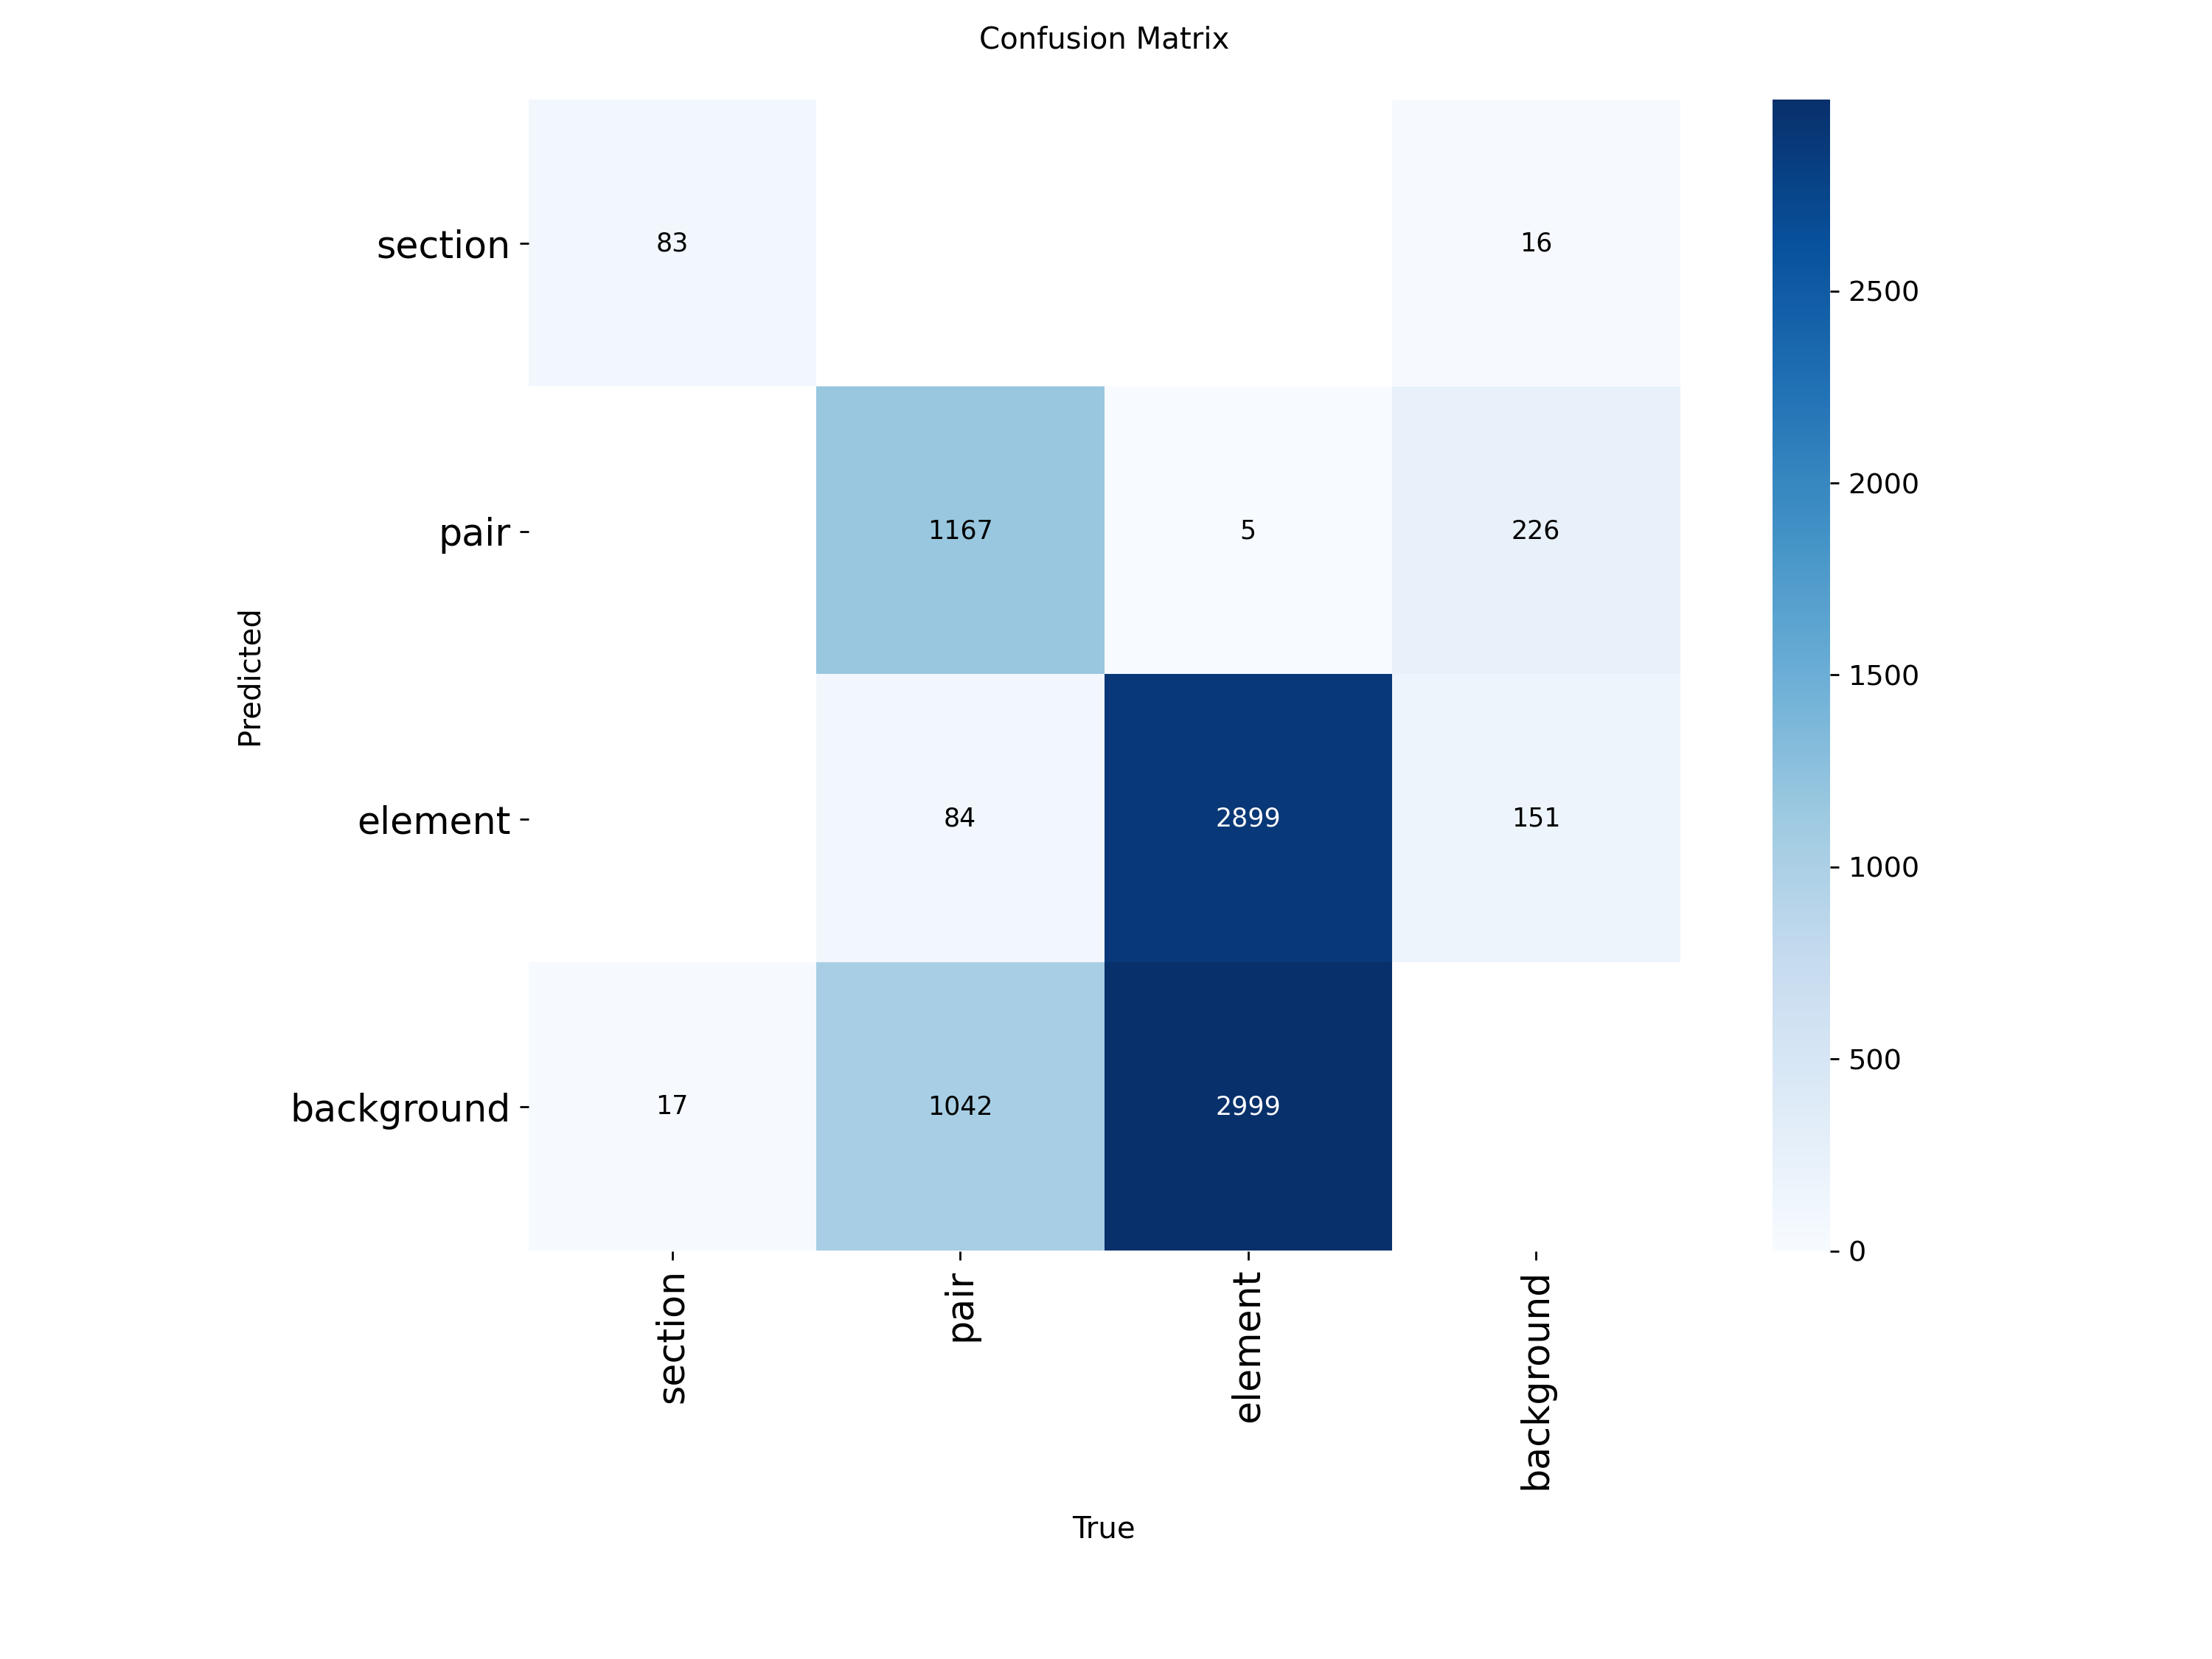
\includegraphics[width=0.95\textwidth]{img/trainings/yolo11s_augmented_lightaug_p50/confusion_matrix.png}
        \caption{confusion matica k najlepšiemu meraniu (augmentácia s počtom epoch 300 a patience 50) - model YOLO11s}
        \label{fig:matrix}
    \end{figure}

    Výsledky ukazujú, že model sa najlepšie vyrovnával s detekciou sekcií, zatiaľ čo detekcia elementov, bola výrazne horšia. Tento problém sa pravdepodobne vyskytoval kvôli nedostatočnému rozlíšeniu malých prvkov, ktoré mohli být ľahko zameniteľné s pozadím. Ďalším faktorom, ktorý mohol ovplyvniť výsledky, je variabilita v štruktúre elementov a párov.

    \begin{figure}[H]
        \centering
        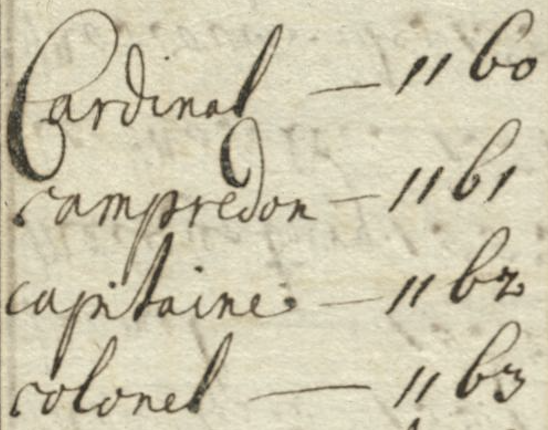
\includegraphics[width=0.95\textwidth]{img/zasahy.png}
        \caption{Niektoré prvky boli ťažko oddeliteľné, čo viedlo k nepresnému označeniu a ťažšiemu rozpoznaniu. Obrázok zo zbierky HLA–HStAM, Best. 4d, (c) HLA–HStAM, f. 4d, Nr. 1223 \cite{HLA1223}}
        \label{fig:zasahy}
    \end{figure}

    \subsection{Diskusia}

    Počas experimentov sa potvrdilo, že detekcia objektov v historických rukopisných dokumentoch prináša výrazné výzvy, pričom významnú úlohu hrajú kvalita datasetu, techniky predspracovania údajov a nastavenie tréningových parametrov.

    Jedno z kľúčových zistení poukázalo na pozitívny vplyv binarizácie dokumentov na presnosť modelu. Výsledky ukázali, že binarizovaný dataset častejšie poskytoval lepšiu výkonnosť než jeho pôvodná, nebinarizovaná verzia. Navyše sa pri binarizácii zaznamenala stabilnejšia konvergencia počas fázy tréningu.

    Ďalšie testovania odhalili dôležitosť správneho nastavenia mechanizmu early stopping. Pri nižších hodnotách parametra patience bol tréning často ukončený predtým, než sa validačné metriky stabilizovali, čo najviac ovplyvnilo výsledky pri datasetoch s augmentáciou. V takýchto prípadoch došlo k výrazným výkyvom validačných metrík počas tréningového procesu.

    Taktiež sa ukázalo, že použitie väčších modelov nemusí vždy viesť k lepším výsledkom pri práci so špecifickými dokumentovými datasetmi. Komplexnejšie modely si vyžadovali značné výpočtové zdroje a niekedy vykazovali horšiu schopnosť generalizácie v porovnaní s menšími a jednoduchšími modelmi.

    Za optimálne riešenie sa ukázalo použitie modelu YOLO11s. Prekvapivo pomohla augmentácia, avšak len v prípade, že bola aplikovaná šetrnejším spôsobom. Naopak, agresívna augmentácia mala tendenciu zhoršovať výsledky, pravdepodobne kvôli nadmernému skresleniu štruktúry dokumentov.
    
    \subsection{Návrhy na možné vylepšenia}
    Na základe získaných výsledkov a identifikovaných limitov možno navrhnúť niekoľko možných vylepšení: 
    \begin{itemize}
        \item Rozšírenie datasetu: Získanie a anotácia ďalších historických dokumentov z rôznych zdrojov by umožnila modelom naučiť sa širšiu škálu vzorov a zvýšila by ich robustnosť. 
        
        \item Rozkúskovanie: YOLO pracuje s degradovanou podobou vstupných obrázkov. Toto má za dôsledok rýchly tréning nenáročný na hardvér, ale zároveň môže zhoršovať schopnosť modelu rozlišovat menšie objekty. Rozkúskovanie obrázkov na menšie časti by mohlo pomôcť zlepšiť detekciu elementov a párov pri zachovaní menšej náročnosti.
        
        \item Výkonnejšia GPU: Trénovanie na výkonnejšej grafickej karte výrazne zvyšuje rýchlosť výpočtov a umožňuje experimentovať s väčším počtom modelov a nastavení.
    
    \end{itemize}
    Tieto návrhy by mohli potenciálne zlepšiť výskum, ktorý by mohol významne prispieť k automatizácii a efektívnemu spracovaniu historických šifrovacích dokumentov.


% Zoznam použitej literatúry
%\bibliographystyle{plain}
%\bibliography{literatura}

% Prílohy (voliteľné)
